\documentclass{pkuthesis}
\newcommand{\preTitleCn}{\zihao{2}}
\newcommand{\preTitleEn}{\zihao{3}}
\newcommand{\titleCn}{奖励塑造的困境破局:基于多选题的强化学习推理研究}
\newcommand{\titleEn}{Reward Shaping Breakthrough:  Enhancing RL Reasoning through Multi-Choice Paradigms}
\newcommand{\studentName}{王昱琛}
\newcommand{\studentID}{2100013153}
\newcommand{\schoolName}{北京大学}
\newcommand{\majorIn}{智能科学与技术}
\newcommand{\tutorName}{冯岩松}
\newcommand{\abstractCn}{随着大语言模型(LLM)在自然语言处理领域的迅猛发展,其在法律推理任务中的应用引起了广泛关注。然而,法律多选题因其答案的非唯一性和推理链条的复杂性,对模型能力提出了更高要求。本文基于中国国家司法考试(JEC-QA)案例分析子集,进行了一系列强化学习推理研究,重点探索了组相对策略优化(GRPO)算法及特定奖励函数(格式奖励与严格完全匹配准确性奖励)的有效性。研究发现,通过精心设计的强化学习策略,即便是直接应用于Qwen-7B-Instruct模型的强化学习(RL Zero),也能取得显著效果。同时,一种融合知识蒸馏监督微调(SFT,以DeepSeek-R1为教师模型)与后续GRPO微调的双阶段训练框架,也达到了与之相当的高性能水平。实验证明,这两种路径均能在JEC-QA测试集上将模型的精确匹配率从0.295大幅提升至0.582。进一步的定量分析与结构化响应评估显示,采用这些强化学习策略后,模型在层次化段落组织、语篇连贯性和法律表述专业性等方面均有显著改进。这些结果凸显了先进强化学习技术(特别是GRPO及针对性的奖励设计)在赋能大语言模型处理复杂专业领域推理任务上的强大潜力。}
\newcommand{\keywordsCn}{大语言模型;法律推理;监督微调;组相对策略优化(GRPO);JEC-QA;多选题;强化学习}
\newcommand{\abstractEn}{
    With the rapid development of Large Language Models (LLMs) in the field of natural language processing, their application in legal reasoning tasks has garnered widespread attention. However, legal multiple-choice questions pose higher demands on model capabilities due to their non-unique answers and complex reasoning chains. This paper, based on the case-analysis subset of the Chinese National Judicial Examination (JEC-QA), conducts a series of research studies on reinforcement learning for legal reasoning, focusing on exploring the effectiveness of the Group Relative Policy Optimization (GRPO) algorithm and specific reward functions (format rewards and strict exact-match accuracy rewards). The study found that with meticulously designed reinforcement learning strategies, even direct reinforcement learning (RL Zero) applied to the Qwen-7B-Instruct model can achieve significant results. Concurrently, a two-stage training framework, integrating knowledge-distilled Supervised Fine-Tuning (SFT, with DeepSeek-R1 as the teacher model) followed by GRPO fine-tuning, also reached a comparably high level of performance. Experiments demonstrate that both pathways can substantially improve the model's exact match rate on the JEC-QA test set from a baseline of 0.295 to 0.582. Further quantitative analysis and structured response evaluation show that after applying these reinforcement learning strategies, the model made significant improvements in hierarchical paragraph organization, textual coherence, and the professionalism of legal expression. These results highlight the strong potential of advanced reinforcement learning techniques, particularly GRPO and targeted reward design, in empowering LLMs to handle complex reasoning tasks in specialized domains.
}
\newcommand{\keywordsEn}{Large Language Models; Legal Reasoning; Supervised Fine-Tuning; Group Relative Policy Optimization (GRPO); JEC-QA; Multiple-Choice Questions; Reinforcement Learning}
\newcommand{\qwen}{Qwen2.5-7B-Instruct}
\newcommand{\deepseekr}{DeepSeek-R1}
\usepackage[style=gb7714-2015]{biblatex}
\usepackage{amsmath}
\usepackage{amssymb}
\addbibresource{ref.bib}
\begin{document}

\section{引言}

\subsection{研究背景}

随着人工智能技术的快速发展,大语言模型(Large Language Models, LLMs)在自然语言处理任务中展现出卓越的性能,尤其在逻辑推理、语义理解和文本生成等方面取得了显著成果。然而,法律领域因其高度的专业性与复杂性,对模型推理能力提出了更高要求。法律问题通常具有非唯一性的特点,涉及多层次的法律逻辑与价值判断,这使得传统强化学习方法在法律任务中的应用面临诸多挑战。目前,主流的大语言模型推理能力多来源于数学与编程领域的训练,而本研究则创新性地探讨通过法律复杂问题训练,促进模型跨领域推理能力的提升。

已有研究表明,传统强化学习方法在面对答案唯一、评价标准明确的任务中表现良好;但在涉及多种合理解释的法律问题中,奖励函数的设计变得尤为困难。具体挑战包括:(1)法律问题的开放性导致标准化的评价指标难以确立;(2)合理答案可能基于不同的法律分析路径或表述方式;(3)法律推理过程通常要求严密的逻辑链条与专业知识支撑。因此,构建有效的法律推理模型,并通过强化学习技术优化其推理路径,成为当前亟需解决的重要科学问题。

近期研究显示,强化学习方法有助于提升大语言模型的推理能力。例如,DeepSeek-RL\cite{guo2025deepseek}、Qwen系列模型\cite{yang2024qwen2} 以及 Seed 系列模型\cite{seed2025seed} 表明,仅通过提供问题与答案对,模型可在缺乏显式推理监督的情况下,通过强化学习自主学习有效的推理策略。然而,这些方法在法律领域的适用性仍待验证,主要原因包括:(1)法律问题评估标准模糊,难以构建可通用的奖励函数;(2)缺乏标准化的评估机制,容易导致模型学习到偏离实际法律逻辑的策略。

为缓解上述问题,本研究选取不定项选择题(Multiple-Choice Questions, MCQs)作为训练数据的基础。该数据形式具有双重优势:一方面,MCQs提供了明确的选项空间,使基于规则的奖励函数设计更为可行;另一方面,多选题要求模型系统性地分析并评估所有选项,有助于培养其更全面的推理能力。本研究采用中国国家司法考试(JEC-QA数据集 \cite{zhong2020jec})中的10,561道案例型多选题作为训练与评估语料,涵盖民法、刑法、诉讼法等主要法律门类,要求模型具备专业级别的法律知识与推理能力。

\subsection{研究目标与贡献}

本研究旨在探索后训练(post-training)策略在法律领域的应用效果,重点关注如何通过强化学习优化大语言模型的法律推理能力。

具体研究目标如下:提升大语言模型在中国国家司法考试多项选择题中的答题准确率与推理质量,使模型能够在法律语境下自主学习并掌握系统的法律推理方法。

为实现上述目标,模型输入格式设计为:
\begin{quote}
    "你是一名法学专家。现在请你解答司法考试中的一道选择题,请你找出所有正确的选项。每道题可能有一个或者多个正确答案。在解答之前,你需要先针对每个提供的选项给出详细的解释。你需要在回答的最后用大括号圈出给出的答案,例如 \{B\} 或者 \{ABD\}。"
\end{quote}

模型输出需包含两个核心部分:
\begin{itemize}
\item \textbf{思考(Reasoning)部分:} 展现完整的法律推理链条,对题目及各选项进行深入分析。
\item \textbf{回答(Answer)部分:} 给出最终选定的选项集合,以指定格式(如 \{A,B\})呈现。
\end{itemize}

本研究的主要贡献包括:
\begin{enumerate}
    \item 提出并验证了一种结合监督微调(SFT)与强化学习(RL)的多阶段训练框架,用于提升大语言模型在复杂法律多选题推理任务中的性能。
    \item 针对法律多选题的特性,设计并评估了多种奖励函数(包括完全匹配、部分匹配及格式奖励),并分析了其对模型行为的影响。
    \item 在真实的中国国家司法考试数据集(JEC-QA案例分析题)上进行了广泛实验,证明了所提方法在提高答题准确率和生成内容结构化方面的有效性。
    \item 对比分析了Zero-RL、SFT以及SFT+RL等不同训练策略,揭示了SFT作为RL冷启动的必要性以及RL在SFT基础上的进一步提升作用。
    \item 深入分析了RL对模型输出结构性特征(如逻辑连贯性、专业表述)的增强效果,为法律人工智能领域的大模型应用提供了实践经验和技术路径。
\end{enumerate}

\subsection{论文结构}

本文采用系统化结构进行组织,各章节安排如下:

\begin{itemize}
    \item \textbf{第二章 相关工作:} 系统梳理大语言模型中强化学习方法的研究进展及其在法律推理任务中的应用现状,并介绍相关数据集。
    \item \textbf{第三章 方法论:} 详细介绍本研究提出的核心方法,重点描述基于多选题的强化学习训练机制,包括任务定义、RLHF流程、PPO、GRPO及其变体(DAPO, Dr.GRPO)等算法,以及奖励函数的基本构成。
    \item \textbf{第四章 实验框架:} 构建实验框架,介绍后训练策略的具体实现,包括基线模型选取、SFT阶段设置、GRPO阶段细节、训练加速框架(DeepSpeed)以及高效推理与RL训练框架(VeRL)等。
    \item \textbf{第五章 实验设计与结果分析:} 呈现详细的实验设计、奖励函数具体实现与对比、不同训练策略(Zero-RL, SFT, SFT+RL)的性能评估,以及对模型输出结构性增强的案例分析。同时,定义了本研究采用的评测指标。
    \item \textbf{第六章 总结与展望:} 总结全文研究成果,分析本方法的优势与局限性,并对未来研究方向进行展望。
\end{itemize}

本研究不仅为法律智能提供了新的技术路径,其提出的混合训练范式与评估框架亦可推广至医疗诊断、金融分析等高专业性的人工智能应用领域。通过构建面向法律推理的大模型训练体系,我们希望推动人工智能向更强逻辑推理能力的方向迈进。

\section{相关工作}


近年来,强化学习(Reinforcement Learning, RL)被广泛应用于大语言模型(Large Language Models, LLMs)的微调与对齐过程中。其中,基于人类反馈的强化学习(Reinforcement Learning from Human Feedback, RLHF)成为主流技术框架,旨在训练奖励模型以捕捉人类偏好,并据此优化语言模型的输出策略。这类方法通常引入额外的奖励函数 $r_{\phi}(x, y)$ 对模型输出进行评分,并通过近端策略优化(PPO)\cite{schulman2017proximal}、直接偏好优化(DPO)\cite{rafailov2023direct} 等策略梯度算法对策略 $\pi_{\theta}(y \mid x)$ 进行更新,从而使模型输出更符合人类预期。这些技术的发展表明,强化学习能够在提升 LLM 可控性和对齐能力方面发挥重要作用。近期的研究也进一步指出,强化学习是引导 LLM 学习推理能力的关键途径。

LLM 的后训练(post-training)技术旨在在通用预训练模型基础上,结合领域数据和任务需求进一步提升模型性能,从而推动了如 DeepSeek-R1\cite{guo2025deepseek} 等大型后训练模型(Large-scale Re-trained Models, LRMs)的发展。这类策略主要包括:使用领域数据进行微调、结合 RLHF 实现人类偏好对齐,以及设计复杂的训练流程以增强模型的多步推理能力。这些方法共同构成了 LLM 从通用能力向领域能力演进的研究范式。

在法律推理智能化研究中,LLM 的应用已经进入纵深发展阶段,但距离司法实践的实际需求仍存在显著能力鸿沟。一方面,法律文本具有强逻辑性,要求模型具备多层级推理能力;另一方面,司法决策强调思维链条的可追溯性与可信度,呼唤模型的思考过程满足 TRACER 标准(Traceable, Reasonable, Accountable, Contextualized, Evidence-based, Rational)。为应对上述挑战,Lawyer LLaMA\cite{huang2023lawyer} 基于 LLaMA 对法律任务进行了微调,表现出对案件分析和法律推理的改进能力;ChatLaw\cite{cui2023chatlaw} 则结合法律知识检索、多专家融合和多智能体方法提升法律场景表现;LawGPT\cite{zhou2024lawgpt} 构建了高质量法律问答数据集,并在中文模型基础上进行了领域特定微调。然而,我们通过系统性分析发现,目前法律大模型普遍采用监督微调(Supervised Fine-Tuning, SFT)这一单一策略,在满足司法场景所需的知识完备性和推理可信度方面仍存显著差距。为此,我们提出融合 SFT 与 RLHF 的双阶段训练框架:首先通过法律数据的监督微调实现法理知识的冷启动,随后引入 RLHF 强化模型的推理能力与知识迁移能力。该混合式训练策略不仅加深模型对法律知识的内化,还显著提升了模型对法条与案例的动态匹配与推理能力,从而提高司法决策的合理性与可解释性。

自 DeepSeek 团队提出 GRPO(Group Relative Policy Optimization)算法以来 \cite{shao2024deepseekmath},其在数学推理等任务中展现出显著性能,但也暴露出训练稳定性差、奖励噪声大等问题。为应对上述挑战,研究者提出了多种改进方法,包括 DAPO(Decoupled Clip and Dynamic Sampling Policy Optimization)\cite{yu2025dapo} 和 Dr. GRPO\cite{liu2025understanding},进一步推动了 RL 算法的发展。

GRPO 的核心机制是通过分组估计(group estimation)方式计算优势函数,从而在无需 critic 模型的情况下降低计算资源消耗,同时保持模型训练的稳定性与高效性。其目标函数可以广义地表示为期望优势的加权和,例如:
\begin{equation}
\text{Objective}_{\text{GRPO-like}} = \mathbb{E} \left[\sum_{t} \text{weighting\_factor}_t \cdot A(s_t, a_t)\right]
\end{equation}
其中优势函数 $A(s_t,a_t)$ 通常基于奖励 
$r(s_t,a_t)$ 和某种形式的基线(如组内平均奖励或价值函数估计 
$V(s_t)$)计算,例如 
$A(s_t,a_t)=r(s_t,a_t)+\gamma V(s_{t+1})-V(s_t)$ 或 GRPO 中的相
对奖励。\text{$weighting\_factor_t$} 可能包含重要性采样比率(如 
$\frac{\pi(a_t|s_t)}{\pi_{\text{old}}(a_t|s_t)}$)及其裁剪版本。

在 GRPO 基础上,DAPO 和 Dr. GRPO 引入如下优化策略:
\begin{itemize}
    \item \textbf{删除 KL 约束}:提升模型自由度,旨在突破参考模型性能上限 \cite{yu2025dapo}。
    \item \textbf{Clip-Higher 策略}:通过非对称裁剪等方式缓解熵崩塌,提高生成多样性 \cite{yu2025dapo}。
    \item \textbf{Token-Level Loss 调整}:通过在所有 token 上计算损失,增强模型对长文本的处理能力,使长序列得到更恰当的权重 \cite{yu2025dapo}。
    \item \textbf{难度偏差修正}:例如,移除标准差归一化处理,以提升指标稳定性 \cite{liu2025understanding}。
    \item \textbf{动态采样机制}:例如,过滤掉组内奖励全为0或全为1的样本,以防止梯度停滞,确保每个样本都能提供有效梯度 \cite{yu2025dapo}。
    \item \textbf{超长奖励重构/长度惩罚}:通过软性惩罚机制规避响应冗长问题,引导模型生成合理长度的回答 \cite{yu2025dapo}。
\end{itemize}

GRPO 系列算法在长文本生成中展现出显著提升,其优化方法为强化学习在语言生成任务中的进一步应用提供了新路径。

\subsection{推理能力与泛化性}

除了 DeepSeek-R1 中提出的 "AHA 时刻"外,强化学习还被发现能在训练过程中自然诱导模型产生自我验证、反思式推理等能力 \cite{el2025competitive}。这类能力在没有明确监督信号的情况下自发出现,表明 RL 具备促进认知过程发展的潜力。

尽管大部分 RL 推理研究集中于数学与代码领域,但已有工作证明 RL 能促进模型向其他结构化或非结构化领域的泛化。例如,Logic-RL\cite{xie2025logic} 通过规则驱动的训练,在逻辑谜题任务中取得成功,并在数学推理任务中迁移表现良好,验证了 RL 能独立于领域知识诱导通用推理机制。

更令人关注的是,一些推理模型(如 DeepSeek-R1\cite{guo2025deepseek})已将推理能力拓展至医学、化学、心理学等人文学科,结合生成式软评分机制处理非结构化答案,为构建跨领域通用推理模型奠定基础。下一步的研究方向包括将此类模型与工具调用、检索增强生成(RAG)等系统集成,OpenAI 最新发布的 o3 模型正朝这一方向迈进。

\subsection{数据集:JEC-QA 案例分析题}

本研究使用中国国家司法考试官方题库中的 JEC-QA 数据集\cite{zhong2020jec},该数据集广泛应用于法律人工智能领域,具有较高的权威性与代表性。

\begin{itemize}
\item \textbf{数据来源}:采自中国国家司法考试历年真题,涵盖民法、刑法、行政法、诉讼法等多个法律分支,具有良好的覆盖性与实用性。
\item \textbf{规模与结构}:
\begin{itemize}
\item 数据集中共包含 26,365 道多项选择题。
\item 每道题可能包含一个或多个正确答案。
\item 题型分为两类:\textbf{知识型问题}(注重法条记忆与直接应用)与 \textbf{案例分析问题}(侧重复杂的法律关系理解与推理)。
\end{itemize}

\item \textbf{研究子集选择}:本研究聚焦于其中 10,561 道 \textbf{案例分析问题}。该题型通常涉及具体案情描述,要求应试者结合相关法律规范进行多步骤的逻辑推理与综合判断,能够充分体现法律推理过程的复杂性。选择该子集的原因在于其更贴近真实法律实践中遇到的复杂情境,对模型的法律理解与深度推理能力提出更高要求。

\item \textbf{数据划分方式}:按照 8:2 的比例将选定的案例分析题划分为训练集与测试集,分别包含 8,449 道与 2,112 道题目,以确保训练的充分性与评估的客观性与代表性。

\item \textbf{任务定义}:模型需完成以下三个关键步骤:
\begin{itemize}
\item 准确识别案情描述中的核心法律争议点。
\item 正确定位并可能需要隐式或显式地结合适用的法律条文或法学原理。
\item 通过多步法律逻辑推理,分析每个选项的正确性,并选出所有正确选项。
\end{itemize}
\end{itemize}

该任务对语言模型的逻辑推理能力、法理理解能力以及语言表达一致性提出了系统性挑战,适合作为评估模型法律智能表现的标准基准。

\section{方法论}

\subsection{任务定义}
本研究旨在提升大型语言模型在中国国家司法考试多项选择题上的法律推理能力与答题准确率。具体任务定义如下:

\begin{itemize}
  \item \textbf{研究目标:}
    提升 LLM 在中国国家司法考试多选题上的法律推理质量及选项预测准确率。
  \item \textbf{输入:}
    一道法律多选题,通常包含一个案例描述和若干备选答案选项。模型被指示先对每个选项进行详细的推理分析。
  \item \textbf{输出:}
    模型的输出应包含两个结构化部分:
    \begin{enumerate}
      \item \emph{思考(Reasoning)}:提供一个完整的法律推理链条,对题干以及各个选项给出详细的解释和分析。
      \item \emph{回答(Answer)}:在推理分析之后,最终以大括号形式给出所有正确选项的集合,例如 "\{B\}" 或 "\{A,B,D\}"。
    \end{enumerate}
\end{itemize}

\subsection{基于人类偏好的强化学习(RLHF)流程概述}
我们采用标准的基于人类反馈的强化学习(Reinforcement Learning from Human Feedback, RLHF)思想来指导模型的微调,尽管在本研究的特定实例化中,我们主要使用基于规则的奖励函数而非直接的人类偏好数据训练奖励模型。广义的RLHF流程包含以下关键步骤:
\begin{enumerate}
    \item \textbf{奖励机制设计/奖励模型训练}:利用预定义的规则(如本研究中的准确性与格式奖励)或人工标注的偏好数据,构建奖励函数或训练奖励模型 $r_{\phi}(x, y)$。该模型/函数基于输入提示 $x$ 和模型生成的回答 $y$,对回答的质量进行评估打分。
    \item \textbf{策略优化}:在奖励信号的指导下,通过策略梯度方法(如PPO、GRPO等)优化语言模型自身的策略 $\pi_{\theta}(y \mid x)$,以提升其生成高质量、高奖励回答的能力。
\end{enumerate}
由于司法考试题目对逻辑一致性和推理链条完整性的要求极高,RLHF(或基于规则的RL)能有效引导模型生成更符合期望的、结构化的解释和答案。

\subsection{近端策略优化(PPO)}
PPO \cite{schulman2017proximal}是一种广泛应用于语言模型强化学习微调的 Actor-Critic 算法。PPO 通过联合训练一个值函数网络(Critic),并引入裁剪代理目标来限制策略更新的幅度,从而提高训练的稳定性和样本效率。其核心思想是通过裁剪重要性采样比率,确保策略更新不会偏离当前策略过远。

\text{PPO 方法}
PPO 是一种基于策略梯度的算法,结合值函数和广义优势估计(Generalized Advantage Estimation, GAE)来计算优势函数 \( \hat{A}_t \),并在奖励中加入 KL 散度惩罚项以稳定训练。其优化目标定义为:
\[
L^{\text{PPO}}(\theta) = \mathbb{E}_{(x, y) \sim D_{\pi_{\text{ref}}}} \left[ r_{\text{model}}(x, y) - \beta \, \text{KL}(\pi_{\theta}(y \mid x) \| \pi_{\text{ref}}(y \mid x)) \right]
\]
其中,\( r_{\text{model}}(x, y) \) 是奖励模型对生成结果 \( y \) 的评分,\( \pi_{\text{ref}} \) 为参考策略(通常为监督微调后的预训练模型),\( \beta \) 为 KL 惩罚系数。策略更新采用裁剪代理目标函数:
\[
L^{\text{CLIP}}(\theta) = \hat{\mathbb{E}}_t \left[ \min \left( r_t(\theta) \hat{A}_t, \, \text{clip}(r_t(\theta), \, 1 - \epsilon, \, 1 + \epsilon) \hat{A}_t \right) \right]
\]
其中,\( r_t(\theta) = \frac{\pi_{\theta}(a_t \mid s_t)}{\pi_{\theta_{\text{old}}}(a_t \mid s_t)} \) 表示当前策略与旧策略在时刻 \( t \) 的概率比,\( \hat{A}_t \) 为 GAE 估计的优势值。然而,PPO 在大规模语言模型中面临两大挑战:一是需要额外训练值函数网络以计算 GAE,增加了参数规模和训练成本;二是文本生成任务中通常仅在序列末尾获得回报信号,导致中间状态的价值估计困难,影响训练的稳定性与效率。为了解决 PPO 在 LM 中需训练 Critic 以及仅末尾奖励的问题,我们引入组相对策略优化(GRPO)方法,该方法以采样组为单位进行相对评价,无需 Critic 结构,且更加稳定高效。

\subsection{组相对策略优化(GRPO)}
GRPO \cite{shao2024deepseekmath}是一种无需值函数的策略优化算法,通过模型自身生成的多组回答样本进行相对评分,估计优势函数(Advantage Function)并更新策略。其主要特点包括:
\begin{enumerate}
    \item \textbf{无需值函数模型}:传统 PPO 依赖值函数 \( V(x) \) 估计优势,而 GRPO 基于策略采样的相对信息,通过组内奖励归一化估计优势,消除了对价值函数的依赖。
    \item \textbf{样本组评分机制}:对于输入 \( x \),从当前策略 \( \pi_{\theta} \) 生成多个回答 \( \{y_1, \dots, y_K\} \),并由奖励模型评分:
    \[
    r_i = r_{\phi}(x, y_i), \quad i = 1, \dots, K
    \]
    根据评分排序,为每个样本分配排名权重 \( \alpha_i \)(如 Softmax 归一化得分),用于构造相对优势。
    \item \textbf{优势函数估计}:
    \[
    A(x, y_i) = \alpha_i - \frac{1}{K} \sum_{j=1}^K \alpha_j
    \]
    其中,\( \alpha_i \) 可为 Softmax 输出或单调映射的排名指标。
    \item \textbf{策略更新目标}:
    GRPO 使用裁剪策略目标限制偏移:
    \[
    L^{\text{GRPO}}(\theta) = \hat{\mathbb{E}}_{(x, y_i) \sim \pi_{\theta_{\text{old}}}} \left[ \min \left( r_{\theta}(x, y_i) A(x, y_i), \, \text{clip}(r_{\theta}(x, y_i), \, 1 - \epsilon, \, 1 + \epsilon) A(x, y_i) \right) \right]
    \]
    其中,\( r_{\theta}(x, y) = \frac{\pi_{\theta}(y \mid x)}{\pi_{\theta_{\text{old}}}(y \mid x)} \)。
\end{enumerate}

\textbf{GRPO 方法}:  
\begin{figure}[h]
    \centering
    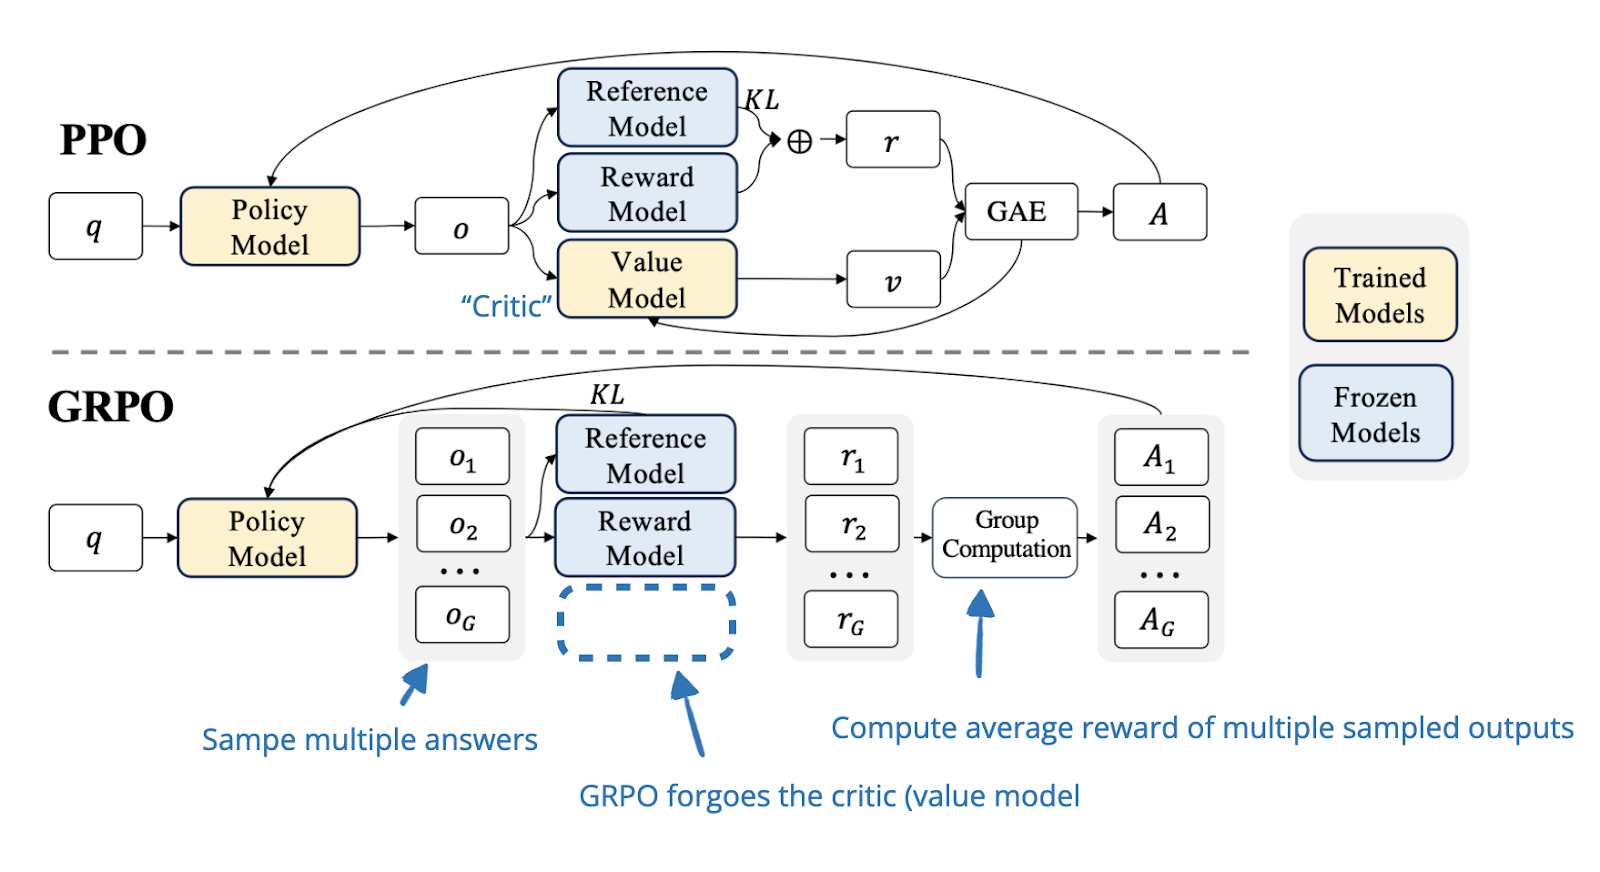
\includegraphics[width=1\textwidth]{figures/grpo.png}
    \caption{GRPO 方法示意图\cite{shao2024deepseekmath}}
    \label{fig:grpo}
\end{figure}
GRPO 通过对输入 \( x \) 生成 \( K \) 个回答 \( \{y_1, y_2, \dots, y_K\} \),利用奖励模型评分 \( r_i = r_{\phi}(x, y_i) \),并应用 Softmax 函数:
\[
\alpha_i = \frac{\exp(r_i / \tau)}{\sum_{j=1}^K \exp(r_j / \tau)}
\]
其中 \( \tau \) 为温度参数。相对优势定义为:
\[
A(x, y_i) = \alpha_i - \frac{1}{K} \sum_{j=1}^K \alpha_j
\]
高于均值的回答获得正优势,反之则为负优势。GRPO 通过组内比较直接评估优势,无需值函数网络,降低了内存和计算开销。


\subsection{DAPO 算法}
为提升模型在长链推理(Chain-of-Thought, CoT)任务中的表现,有工作引入了\textbf{解耦裁剪与动态采样策略优化(Decoupled Clipped and Dynamic Sampling Policy Optimization, DAPO)}算法\cite{yu2025dapo}。该算法通过一系列创新策略,优化了模型在复杂推理任务中的训练效率和性能。以下是其核心创新点的详细描述:

\begin{itemize}
    \item \textbf{解耦裁剪策略}:
    DAPO 采用非对称裁剪机制,分别设置下限 \( \varepsilon_{\text{low}} = 0.2 \) 和上限 \( \varepsilon_{\text{high}} = 0.28 \)。在传统的 PPO-clip 算法中,裁剪参数 \(\varepsilon\) 是对称的,即上下限相同,这限制了低概率动作(exploration token)的提升空间。DAPO 通过解耦上下裁剪参数,允许低概率动作的提升幅度更大,从而促进模型的多样性。具体而言,对于策略更新的裁剪目标函数 \(L^{CLIP}\),DAPO 定义为:
    \[
    L^{CLIP} = \mathbb{E}_{t} \left[ \min \left( \frac{\pi(a_t|s_t)}{\pi_{\text{old}}(a_t|s_t)} A^{\pi_{\text{old}}}(s_t, a_t), \; \varepsilon_{\text{high}} \right) - \max \left( \frac{\pi(a_t|s_t)}{\pi_{\text{old}}(a_t|s_t)} A^{\pi_{\text{old}}}(s_t, a_t), \; -\varepsilon_{\text{low}} \right) \right]
    \]
    其中,\(\pi(a_t|s_t)\) 是当前策略,\(\pi_{\text{old}}(a_t|s_t)\) 是旧策略,\(A^{\pi_{\text{old}}}(s_t, a_t)\) 是优势函数。这种非对称裁剪机制能够有效避免熵崩溃现象,同时提升模型的探索能力。

    \item \textbf{动态样本重采样}:
    DAPO 通过过采样并筛选出准确率非 0 或 1 的样本,确保每个样本都能提供有效的梯度信息。在传统的采样方法中,组内全对或全错的样本会导致优势函数为零,从而没有梯度,影响训练效率。DAPO 的动态采样策略通过过滤这些极端样本,确保每个采样组内的优势函数均非零。具体而言,对于采样组 \(G\),DAPO 仅保留满足 \(0 < \text{accuracy}(G) < 1\) 的样本组,从而提高训练效率并降低梯度方差。

    \item \textbf{Token 级策略梯度损失}:
    DAPO 在所有 token 上计算损失,赋予长序列更大的权重。传统的样本级损失计算方式(sample-level loss)对长回答和短回答赋予相同的权重,这在长链推理任务中是不合理的。DAPO 采用 token 级损失计算方式,定义为:
    \[
    L^{TOKEN} = \sum_{t=1}^{T} \log \pi(a_t|s_t) \cdot A^{\pi_{\text{old}}}(s_t, a_t)
    \]
    其中,\(T\) 是序列长度。通过这种方式,DAPO 对长回答中的高质量和低质量响应模式赋予更大的权重,从而提升模型在复杂推理任务中的表现。

    \item \textbf{过长奖励整形}:
    DAPO 采用软长度惩罚机制,其奖励函数定义为:
    \[
    R_{\text{length}}(y) = \begin{cases} 
    0, & |y| \leq L_{\text{max}} - L_{\text{cache}} \\ 
    \frac{(L_{\text{max}} - L_{\text{cache}}) - |y|}{L_{\text{cache}}}, & L_{\text{max}} - L_{\text{cache}} < |y| \leq L_{\text{max}} \\ 
    -1, & L_{\text{max}} < |y|
    \end{cases}
    \]
    其中,\(L_{\text{max}} = 16384\) 是最大允许长度,\(L_{\text{cache}} = 4096\) 是缓存长度。这种软惩罚机制能够有效惩罚过长的回答,同时避免因长度限制而引入的噪声。具体而言,当回答长度 \(|y|\) 超过 \(L_{\text{max}} - L_{\text{cache}}\) 时,奖励函数逐渐减小,直至达到最大长度 \(L_{\text{max}}\) 时,奖励值为 \(-1\)。这种机制能够引导模型生成更合理的回答长度,同时避免因长度限制而带来的梯度消失问题。
\end{itemize}


\subsection{Dr.GRPO 算法}
\textbf{Dr.GRPO 算法}\cite{liu2025understanding}是对 GRPO 的改进,通过修正偏见提升推理能力。其主要改进包括:
\begin{itemize}
    \item \textbf{去除响应长度偏见}:移除除以响应长度的项,确保策略更新不受长度影响。
    \item \textbf{消除问题难度偏见}:移除组内奖励标准差归一化,使学习过程更平衡。
    \item \textbf{调整基线计算}:优化基线估计为:
    \[
    \mathbb{E}[r_k] = \frac{1}{K} \sum_{k=1}^K r_k
    \]
\end{itemize}
目标函数为:
\[
J_{\text{Dr.GRPO}}(\theta) = \mathbb{E}_{\{\tau_k\}_{k=1}^K \sim \pi_{\theta_{\text{old}}}}\left[\sum_{k=1}^{K} \sum_{t=1}^{|o_k|} \hat{\rho}_{k,t}(\theta) (r_k - \mathbb{E}[r_k])\right]
\]

\subsection{方法小结}
本研究首先清晰定义了面向法律领域的多项选择题推理任务,明确了模型的输入输出格式,旨在引导模型生成结构化的、包含明确推理过程的法律分析。我们采用了基于强化学习的后训练(post-training)框架来提升预训练语言模型的性能。在此框架下,我们从经典的PPO算法出发,分析了其在处理复杂文本生成任务(尤其是长链法律推理)时可能遇到的挑战,如对Critic网络的依赖和对稀疏奖励信号的敏感性。
随后,我们重点引入了无需Critic的GRPO方法及其变体(如DAPO和Dr.GRPO)。GRPO通过比较同一输入下模型生成的多个候选输出的相对好坏来估计优势,简化了训练流程并有望提升训练效率和稳定性。DAPO和Dr.GRPO则在GRPO的基础上,针对长链推理、样本效率、梯度偏差等问题进行了进一步的优化。
核心奖励函数的设计结合了格式奖励(确保输出结构的合规性)和准确性奖励(确保法律判断的正确性),以期在提升模型专业能力的同时,保证其输出的可用性和可解释性。整个方法论旨在构建一个能够有效学习并执行复杂法律推理任务的智能系统。

\subsection{奖励函数设计原则}
在本研究中,奖励函数的设计是强化学习成功的关键。我们主要关注两类奖励:格式奖励和准确性奖励,这些在实验部分的第 \ref{sec:reward_design_experimental} 节有更详细的定义和评估。此处简述其设计理念。

\textbf{格式奖励 (Format Reward)}

格式奖励的核心目标是引导模型生成符合预设结构规范的输出,这对于提升法律文书的可读性、一致性和专业性至关重要。我们要求模型的输出包含明确的结构标签,如 \texttt{<思考>} 和 \texttt{<回答>},用以清晰地分隔模型的推理过程和最终结论 \cite{guo2025deepseek}。例如,在法律问题解答中,\texttt{<思考>} 部分应详细阐述对案情的分析、相关法律条文的援引、不同法律概念的辨析等;而 \texttt{<回答>} 部分则应简洁明了地给出最终的选项。通过施加格式奖励,可以促使模型学习并遵循这种结构化的表达方式。

\textbf{准确性奖励 (Accuracy Reward)}

准确性是评价法律推理模型核心性能的指标。与单项选择题相比,不定项选择题(一个或多个正确答案)对模型的推理能力提出了更高要求。单选题可能因为选项空间有限,允许模型通过不完全或表面的推理侥幸答对。而不定项选择题则要求模型全面评估每个选项的正确性,排除了猜测或片面推理的可能性,更能有效训练模型强大的、全面的推理能力,尤其是在法律这样逻辑严密的复杂领域。

因此,我们设计了严格的准确性奖励机制。令 $S_{\text{true}}$ 为多选题的标准答案选项集合,$S_{\text{pred}}$ 为模型预测的选项集合。准确性奖励 $R_{\text{accuracy}}$ 的一个核心形式是"完全匹配奖励":
$$ R_{\text{accuracy}}(S_{\text{pred}}, S_{\text{true}}) = \begin{cases} 1 & \text{if } S_{\text{pred}} = S_{\text{true}} \\ 0 & \text{otherwise} \end{cases} $$
这种机制确保只有当模型完整且准确地选出所有正确选项,并排除所有错误选项时,才能获得正向反馈。它激励模型追求推理的深度和广度,避免基于捷径的、不完整的解决方案,从而迫使模型对当前任务形成更深刻、更全面的理解。此外,如第 \ref{sec:reward_design_experimental} 节所述,我们还探索了"部分匹配奖励"以提供更细粒度的反馈。


\section{实验框架}


\subsection{基线模型(Baselines)}

为全面评估所提方法的有效性,我们选取了以下基线模型进行对比:
\begin{itemize}
\item \textbf{\qwen}:作为当前中文领域表现最强的开源语言模型之一\cite{yang2024qwen2},该模型被用于评估其在目标法律任务上的 zero-shot 能力。这代表了通用预训练模型在未经特定法律领域微调时的原始性能参考。
\item \textbf{R1 蒸馏模型(SFT蒸馏基线)}:我们首先使用教师模型 (\deepseekr) 对JEC-QA数据集生成高质量的推理 odpowiedzi。然后,我们将这些生成结果(包含推理过程和答案)作为蒸馏数据,对学生模型(\qwen)进行监督微调(SFT)。这种做法受到了近年来在数学和编程等复杂推理任务中取得显著成效的 teacher-student 知识蒸馏范式的启发\cite{guo2025deepseek}。该模型代表了仅通过SFT(使用高质量蒸馏数据)所能达到的性能水平,作为后续强化学习阶段的有力起点和对比基线。

\end{itemize}

\subsection{监督微调(SFT)阶段}

我们采用 LLaMA-Factory 和 DeepSpeed 作为监督微调(SFT)的主要训练框架。LLaMA-Factory 是一个专为大型语言模型微调而开发的高效易用工具集,它支持包括全参数微调、LoRA/QLoRA等参数高效微调方法,以及多GPU并行训练等功能\cite{llamafactory}。在本研究中,我们主要利用LLaMA-Factory来组织和管理模型的全参数微调流程。

在蒸馏实验的SFT设置中,我们首先基于 \texttt{jec-qa-1-multi-choice} 数据集的训练部分,使用教师模型 \deepseekr 生成的带有详细思考过程和答案的样本作为"黄金"教师信号,构建了高质量的蒸馏语料库。随后,利用该蒸馏语料对学生模型 \qwen 进行全参数监督微调。训练过程采用以下关键超参数设置:训练轮次(epochs)设定为 2,批处理大小(batch size)为 32,最大上下文长度(max context length)为 4096 tokens,学习率(learning rate)设定为 $1 \times 10^{-5}$。学习率调度采用余弦退火策略(cosine decay schedule),并在总训练步骤的前 10\% 进行学习率预热(warm-up)。这些超参数的选取综合考虑了任务的复杂度、模型的容量以及已有研究的经验,旨在提升训练过程的收敛性和稳定性,并充分学习教师模型的知识。

\subsection{GRPO 阶段}

在监督微调(SFT)阶段之后,我们进一步对经过SFT优化的 \qwen 模型执行GRPO(Group Relative Policy Optimization)训练。此阶段的核心在于通过强化学习进一步提升模型的推理能力和答案选择的准确性。该阶段的奖励函数设计结合了以下两项关键指标:
\begin{itemize}
\item \textbf{准确性奖励(Accuracy Reward)}:根据模型输出的最终选项集合与标准答案选项集合的匹配程度进行计算。我们实验了包括"完全匹配奖励"和"部分匹配奖励"在内的多种形式(详见第 \ref{sec:reward_design_experimental} 节)。
\item \textbf{格式奖励(Format Reward)}:旨在鼓励模型输出符合预设规范的结构化响应,例如包含清晰的"思考"和"回答"部分,并确保答案格式的统一性。
\end{itemize}
通过精心设计这种多维度的奖励信号,我们旨在引导模型在生成法律问题解答的过程中,不仅追求法律结论的正确性,同时也兼顾答案呈现的逻辑性和规范性,从而更好地适应实际法律应用场景的需求。

\subsection{训练加速框架:DeepSpeed 与 ZeRO 策略}
为了高效地训练大规模语言模型,我们使用 DeepSpeed 作为底层的训练加速库。DeepSpeed 是由微软研究院推出的一款功能强大的分布式训练优化库,其核心技术之一是 ZeRO(Zero Redundancy Optimizer)系列优化策略。ZeRO通过在分布式训练环境中对模型训练过程中的三个关键部分——优化器状态(Optimizer States)、梯度(Gradients)以及模型参数(Model Parameters)——进行智能化的分区和管理,从而大幅降低了单张GPU的显存需求,并显著提升了训练的规模和效率。ZeRO策略通常分为三个主要阶段:
\begin{itemize}
\item \textbf{ZeRO Stage 1}:主要对优化器状态进行分区。每个GPU只负责更新和存储其对应参数分片的优化器状态,从而将优化器状态的显存消耗降低N倍(N为GPU数量)。
\item \textbf{ZeRO Stage 2}:在Stage 1的基础上,进一步对梯度进行分区。在反向传播计算出梯度后,梯度也会被分散到各个GPU上,每个GPU只保留其负责更新参数的那部分梯度,进一步减少显存占用。
\item \textbf{ZeRO Stage 3}:在前两个阶段的基础上,最终对模型参数本身也进行分区。这意味着每个GPU只持有模型参数的一个片段。这是ZeRO系列中内存优化程度最高的阶段,特别适用于训练参数量远超单卡显存容量的超大规模模型。
\end{itemize}
通过采用DeepSpeed及其ZeRO优化策略(本研究中可能根据具体硬件和模型大小选择合适的Stage),我们能够在有限的硬件资源条件下,对7B参数级别的大型语言模型进行高效的全参数微调和强化学习训练。

\subsection{VeRL:高效推理与强化学习训练框架}
除了模型训练框架,推理阶段的高效引擎以及面向强化学习的高效训练框架也是研究的热点。

\textbf{vLLM与高效推理:} vLLM 是一个专为 LLM 推理设计的高吞吐量、低延迟服务库。它通过引入创新性的内存管理技术,如分页注意力(PagedAttention),有效解决了传统注意力机制中KV缓存的浪费问题。PagedAttention允许KV缓存在物理非连续的内存块中存储,类似于操作系统中的虚拟内存分页机制,从而显著减少了内存碎片,提高了GPU内存的利用率。实验结果表明,与传统的HuggingFace Transformers和OpenAI TGI等框架相比,vLLM在相同硬件资源下可实现数倍以上的吞吐量提升,同时大幅减少KV缓存浪费。vLLM支持多种主流模型架构(如LLaMA、Mistral、Qwen、DeepSeek等),并提供量化与工具调用等扩展功能。这些优化使得在法律等领域部署大型LLM进行在线服务或大规模批处理推理时,效率和可扩展性得到显著提高。

\textbf{VeRL框架概述与核心概念:} \\
VeRL是一款面向RL的高效训练框架,它针对大模型强化学习的特性进行了深度优化。
\begin{enumerate}
    \item \textbf{RL与SFT的核心差异}:
    从自然语言处理(NLP)的视角来看,RL 与传统的监督微调(SFT)主要有以下差异:
    \begin{itemize}
        \item \textbf{引入奖励与惩罚信号}:SFT 主要通过模仿高质量的标注数据(正例)进行学习。而RL则引入了奖励机制,对模型生成的优质样本给予正向奖励,对劣质样本施加负向奖励或不奖励。无论是策略梯度方法、GRPO、Reinforce 还是 PPO,其核心都在于如何设计奖励函数的具体形式、惩罚的颗粒度(token级、宏操作级、序列级等)以及奖励信号的强度与平滑性(例如,是否使用基线(baseline)进行中心化、是否加入KL散度约束以限制策略漂移、是否使用裁剪(clip)技巧等)。
        \item \textbf{允许模型自采样并进行在线训练}:SFT 通常依赖于静态的人工标注数据集或其他模型预先生成的数据(如知识蒸馏)。相比之下,RL 允许模型根据当前策略与环境(或自身生成的输出)进行交互,实时采样新的经验数据,并利用这些新数据在线地更新和优化自身策略。
    \end{itemize}

    \item \textbf{On-policy vs. Online Learning}:
    \begin{itemize}
        \item \textbf{Online Learning (在线学习)}: 指的是当前策略能否与环境进行实时交互并即时获取奖励信号。例如,在数学问题求解任务中,模型生成解题步骤后可以立即通过外部验证器得知答案是否正确并获得奖励。在如图形用户界面(GUI)Agent或自动驾驶等需要复杂模拟环境的场景中,构建高效的模拟器是实现在线学习的关键。
        \item \textbf{On-policy Learning (同策略学习)}: 指的是用于训练模型的数据必须是由当前正在优化的最新策略所采样得到的。在实际操作中,为了提高训练效率,常常会预先采样大量的经验数据,然后将这些数据分成多个小批量(mini-batch)进行多轮更新。在这种情况下,严格来说,除了第一个mini-batch是严格on-policy的,后续的mini-batch都是基于一个略微过时的策略(相对于当前正在更新的策略而言)采样的,因此属于近似on-policy或某种程度的off-policy。
    \end{itemize}
    常用的 GRPO、Reinforce、PPO 等方法通常被设计为 \emph{online} 学习算法,但它们是否严格 \emph{on-policy} 则取决于具体的实现细节,特别是mini-batch的数量和经验回放(experience replay)的使用情况。

    \item \textbf{Ray 系统概览}:
    Ray 是一套用于构建和运行分布式应用程序的开源计算框架。它为 VeRL 和 OpenRLHF 等强化学习框架提供了底层的 Actor 模型管理、任务调度以及资源分配能力。其核心概念包括:
    \begin{itemize}
        \item \textbf{Ray Actor}: 是一个有状态的远程计算单元,通过 \texttt{@ray.remote} 装饰器修饰Python类来定义。每个Actor在运行时对应一个独立的进程,拥有自己的内部状态(注意:这里的"Actor"是Ray框架的术语,与RL中的"Actor"角色,即策略网络,是不同概念,尽管RL的Actor角色可以实现为一个Ray Actor)。
        \item \textbf{Ray Task}: 是一个无状态的远程函数调用,通过 \texttt{@ray.remote} 装饰器修饰Python函数来定义。Ray Task的执行是无状态的,其局部变量对任务提交方不可见。
        \item \textbf{资源管理}: Ray 能够根据任务需求(如CPU、GPU、内存等)进行自动化的资源调度。它还支持 \textit{placement group} 的概念,允许用户将一组相关的Ray Actor或Task固定在同一台或不同组的设备(bundle)上执行,以优化通信或满足特定的硬件亲和性需求。
        \item \textbf{异步执行}: Ray 的任务调度默认是异步的。当一个Ray Task或Actor方法被调用时,它会立即返回一个对象引用(future),而实际的计算则在后台的某个worker上执行。用户可以使用 \texttt{ray.get()} 来阻塞等待并获取结果,或使用 \texttt{ray.wait()} 来非阻塞地轮询一组任务的完成状态。
    \end{itemize}
    在RL训练中引入异步设计,可以有效地让Actor(策略网络)、Critic(价值网络)、Generator(数据生成器)、RM(奖励模型)等不同角色的计算过程实现流水线式的重叠执行。例如,当Actor网络正在使用上一批收集到的数据进行参数更新时,Generator可以并行地使用当前的策略生成下一批训练样本。鉴于o1风格的RL(可能指需要大量rollout的RL范式)的主要性能瓶颈通常位于rollout阶段(即数据生成阶段),未来的优化方向之一是更充分地异步化rollout过程,例如在夜间或集群空闲时段充分利用线上推理集群的算力进行数据预生成。

    \item \textbf{并行策略 (Parallelism Strategies)}:
    \begin{itemize}
        \item \textbf{3D 并行及扩展}: 大语言模型的训练(如Megatron-LM框架)和推理引擎(如vLLM、SGLang)已经广泛支持数据并行(Data Parallelism, DP)、张量并行(Tensor Parallelism, TP)和流水线并行(Pipeline Parallelism, PP)这三种主要的并行技术,合称3D并行。VeRL 在新版本中基于 Ulysses 等技术进一步支持了序列并行(Sequence Parallelism, SP),这对于处理长文本序列的强化学习任务尤为关键,因为它可以在序列维度上对计算和内存进行切分。
        \item \textbf{混合并行与优化}: 不同的RL角色(Actor, Critic, RM等)在训练的不同阶段(如rollout、训练、评估)可能对并行策略有不同的需求。VeRL 借助其 \emph{hybrid engine} 对这些并行策略的组合进行了诸多优化,例如实现了零冗余参数的重新分片(re-sharding),以在不同并行配置间高效切换。
    \end{itemize}


    \item \textbf{FSDP 与 Megatron 的对比与兼容}:
    FSDP(Fully Sharded Data Parallelism,由Meta提出)和 Megatron-LM(由NVIDIA提出)代表了两种主流的分布式训练框架设计理念:
    \begin{itemize}
        \item \textbf{FSDP}: 其核心思想是将模型的参数、梯度以及优化器状态在数据并行的各个GPU之间进行完全分片存储。每个GPU只持有完整模型的一部分,仅在需要时通过通信获取其他部分。FSDP通常与计算和通信的重叠执行相结合,其设计逻辑相对清晰,更容易支持新的模型结构,因此被认为对研究更为友好。
        \item \textbf{Megatron-LM}: 主要通过张量并行和流水线并行来实现模型并行,在训练数十亿甚至数百亿参数的超大模型时展现出较强的性能优势。其参数重新分片(re-sharding)的开销相对较低,更偏向于极致性能和工程优化。
    \end{itemize}
    VeRL 框架设计为同时兼容这两种主流的分布式训练引擎,为用户提供了灵活性。
\end{enumerate}

\subsubsection{VeRL 相关核心概念 (VeRL-related Concepts)}
\paragraph{混合流程 (Hybrid Flow)}
强化学习的训练逻辑通常涉及多个模型(Actor, Critic, Reward Model, Reference Model等)之间的复杂交互和数据流动。VeRL 将这种数据流抽象为两个层面:
\begin{itemize}
    \item \textbf{控制流 (Control Flow)}: 位于较高层次,描述了不同RL角色之间的交互逻辑和执行顺序。例如,Actor生成经验数据后,Critic和Reward Model分别对这些经验进行评估打分,Reference Model可能用于计算KL散度,然后这些信息汇总后用于计算广义优势估计(GAE)和最终的损失函数。
    \item \textbf{计算流 (Computation Flow)}: 位于较低层次,描述了单个RL角色内部的具体计算过程,如模型的前向传播、反向传播、优化器更新步骤,以及自回归生成(对于Actor)等。
\end{itemize}

\paragraph{单控制器 vs. 多控制器 (Single Controller vs. Multiple Controllers)}
\begin{itemize}
    \item \textbf{单控制器 (Single Controller)}: 指由一个中心的控制器统一管理所有子模块(RL角色)的执行和协调。这种架构通常逻辑清晰,易于理解和维护。VeRL 在实现RL算法的整体\emph{控制流}时采用了单控制器模式,这极大地便利了新算法的开发和调试。
    \item \textbf{多控制器 (Multiple Controllers)}: 指将控制逻辑分散到多个并行的控制器中,这些控制器可能通过集合通信(collective communication)等方式进行同步。这种模式的潜在优势是降低了单点控制的通信开销,但逻辑实现上可能更为复杂。VeRL 在其\emph{计算流}的维度(例如,一个RL角色的分布式执行)则可能采用类似多控制器的模式(例如,每个GPU上运行一个worker,它们协同完成计算任务),以降低节点内或节点间的通信负载。
\end{itemize}
VeRL 通过设计多层级的 Worker 结构(例如,\texttt{RayWorkerGroup} $\rightarrow$ \texttt{WorkerDict} $\rightarrow$ \texttt{ModelWorker} $\rightarrow$ \texttt{ParallelWorker})来封装和管理复杂的计算流。

\paragraph{混合引擎 — 模型放置策略 (Hybrid Engine — Model Placement Strategy)}
在多模型RL训练中,如何将不同的模型(Actor, Critic, RM等)放置到可用的计算设备(如GPU)上是一个关键问题。VeRL 的混合引擎支持灵活的模型放置策略:
\begin{enumerate}
    \item \textbf{分开放置 (Separate Placement)}: 每个RL角色(或其副本)独立占用一组设备。这种方式允许角色之间完全异步执行,但如果某些角色的计算量较小或空闲时间较长,可能会导致GPU利用率偏低。
    \item \textbf{分组放置 (Grouped Placement)}: 将某些计算上可以重叠或逻辑上紧密相关的角色分组放置到同一组设备上。这样做既能利用计算的重叠来提高效率,又能减少设备空闲。
    \begin{itemize}
        \item 典型的分组策略可能包括:Actor(策略模型)和Generator(用于生成经验的推理模型,通常是Actor的副本)放在同一组设备上,因为它们需要实时同步参数。而Critic、Reward Model 和 Reference Model 则可以根据其计算需求分别放置或与其他模型组合。
    \end{itemize}
    \item \textbf{全部共置 (Collocated Placement)}: 将所有RL角色都放置在同一组(甚至同一张)设备上,并分时复用设备资源。这种方式可以最大化单一设备的占用率,但所有角色基本上只能串行执行,限制了并行度。
\end{enumerate}
VeRL 通过引入 \texttt{resource pool} 的概念来灵活支持以上各种放置策略,并设计了 \texttt{worker\_dict} 这样的数据结构来动态管理不同角色模型的加载(\texttt{reload\_params})和卸载(\texttt{offload\_params}),以适应不同的计算阶段和资源配置。

\paragraph{数据传输协议 (Data Transfer Protocol)}
为了适配不同RL角色(Actor, Critic等)对数据并行切分(sharding)和重组(reshaping)的不同需求,VeRL 设计了一套统一的数据分发(Dispatch)与收集(Collect)协议。这些协议可以方便地以Python装饰器的形式绑定到Worker的方法上,从而对用户透明地实现复杂的数据流管理和执行模式控制。

\paragraph{训练流程示意 (Training Flow Illustration)}
一个典型的VeRL训练迭代步骤可能如下:
\begin{enumerate}
    \item \texttt{RayPPOTrainer} (或 \texttt{GRPOTrainer} 等具体的RL算法训练器) 向其管理的 \texttt{RayWorkerGroup} (一组执行RL任务的Ray Actor) 发送方法调用指令(例如,执行一次rollout,或进行一次训练更新)。
    \item \texttt{RayWorkerGroup} 接收到指令后,首先会根据预设的数据分发协议将输入数据(如prompts)分发给组内的各个Worker。然后,根据当前配置的执行模式(例如,是所有Worker都执行同一个任务,还是每个Worker执行不同的任务),决定哪些Worker实际执行该任务。
    \item Worker执行完毕后,其产生的结果(例如,生成的序列、计算出的梯度等)会经过相应的收集逻辑进行处理和汇总,最终返回给Trainer。
\end{enumerate}

\subsubsection{RL 设置:VeRL中GRPO的实现}
本研究的强化学习阶段采用 VeRL(Sheng et al., 2024,假设的引用)框架来实现组相对策略优化(GRPO)。以下结合 VeRL 的特性,详细阐述 GRPO 在本研究中的具体实现步骤。

\paragraph{1. 初始化与核心组件}
GRPO 的训练流程由 VeRL 中的 \texttt{GRPOTrainer} (或类似命名的类) 进行统一管理和调度。在初始化阶段,需要配置以下核心组件:
\begin{itemize}
    \item \textbf{策略模型(Actor)}: 即需要优化的语言模型。在本研究中,采用的是经过SFT预热的 \qwen 模型。
    \item \textbf{参照模型(Reference Model)}: 通常是与Actor同架构的、在SFT阶段固定下来的模型。其主要作用是计算KL散度惩罚项,以限制Actor策略在更新过程中与初始(或某个稳定)策略的偏离程度,有助于稳定训练。
    \item \textbf{奖励函数 (Reward Function)}: 在本研究中,由于目标是法律选择题,奖励函数主要基于规则设计,包括格式奖励和准确性奖励(详见第 \ref{sec:reward_design_experimental} 节)。这避免了训练一个独立的、基于人类偏好数据的奖励模型(Reward Model, RM)的复杂性,但VeRL框架本身也支持集成外部RM。
\end{itemize}

\paragraph{2. Rollout(经验/数据生成)阶段}
\begin{itemize}
    \item \textbf{权重同步 (Weight Synchronization)}: 在每一轮(或每N轮)大的迭代开始之前,需要将Actor模型最新的参数权重同步到用于生成经验的推理引擎(例如,vLLM 或 SGLang,如果VeRL集成了这些引擎)。VeRL中可能通过 \texttt{RolloutShardingManager} 或类似的组件来高效管理和分发这些权重。
    \item \textbf{提示采样 (Prompt Sampling)}: 从训练数据集中(如JEC-QA的训练子集)抽取一批次的prompts(即选择题的题干和选项描述)。
    \item \textbf{序列生成 (Sequence Generation)}: \texttt{GRPOTrainer} 调用其内部的生成模块(例如,通过 \texttt{generate\_sequences} 方法驱动推理引擎),让当前的Actor策略针对每个prompt并行生成 $K$ 条不同的候选响应(response)。在本研究中,设置 $K=7$,并通过设置较高的温度参数(如 \texttt{temperature=1.0})来鼓励生成多样化的输出。
    \item \textbf{奖励计算 (Reward Computation)}: 对于生成的每一条响应,使用预定义的规则奖励函数(格式奖励 + 准确性奖励)进行评分,得到 $r_i$。
    \item \textbf{数据封装与存储 (Data Encapsulation and Storage)}: 将每个prompt、其对应的 $K$ 条响应、每条响应在生成时(由Actor策略给出)的token级对数概率(log probabilities)、注意力掩码(mask)以及计算得到的奖励值 $r_i$ 等信息封装成经验数据单元。这些经验数据将组成后续策略更新阶段的训练批次。本研究中,prompt的最大长度设置为512 tokens,生成的响应最大长度设置为2048 tokens。
\end{itemize}

\paragraph{3. 对数概率计算 (Log Probability Computation)}
为了计算PPO或GRPO中的策略比率(importance sampling ratio),需要获取新旧策略对生成序列的对数概率:
\begin{itemize}
    \item \textbf{旧策略对数概率 ($\text{old\_log\_prob}$)}: 这是指在进行当前一轮策略参数更新之前,生成当前这批经验数据时所用的那个版本的Actor策略($\pi_{\theta_{\text{old}}}$)对这些数据((prompt, response)对)给出的token级对数概率。这些值通常在rollout阶段就计算并保存下来。然而,有时高性能推理引擎可能不直接保存完整的token-level log-prob,或者保存的值可能受到数值波动或特定并行策略的影响。因此,一种常见的做法是,在训练开始前,使用未更新的Actor(即$\theta_{\text{old}}$)对收集到的(prompt, response)样本对再次进行一次前向传播,以精确获取$\text{old\_log\_prob}$。
    \item \textbf{参照策略对数概率 ($\text{ref\_log\_prob}$)}: 使用Reference Model对同一批经验数据((prompt, response)对)进行前向传播,计算其token级对数概率。这些概率用于计算KL散度惩罚项 $KL(\pi_{\theta} || \pi_{\text{ref}})$。在第一轮迭代时,如果Reference Model就是SFT模型,那么$\text{ref\_log\_prob}$可能与初始的$\text{old\_log\_prob}$相同。
\end{itemize}

\paragraph{4. 奖励与优势估计 (Reward and Advantage Estimation)}
\begin{itemize}
    \item \textbf{奖励整合 (Reward Aggregation)}: VeRL框架允许灵活集成奖励来源,可以是外部训练的RM,也可以是用户自定义的奖励函数。本研究采用的是后者,即基于规则的格式与准确性奖励。
    \item \textbf{优势函数计算 (Advantage Function Computation)}: \texttt{GRPOTrainer} 调用其内部的 \texttt{compute\_advantage} (或类似) 方法。依据GRPO的核心思想(如本文方法论部分的公式所示),在每个prompt对应的 $K$ 个样本组内部计算相对优势。这通常涉及到计算组内奖励的均值或中位数作为基线,然后用每个样本的奖励减去该基线得到优势值。VeRL可能还提供选项对计算出的优势进行标准化处理(例如,通过 \texttt{norm\_adv\_by\_std\_in\_grpo} 配置项,将优势值除以其在组内或批次内的标准差),以稳定训练。
\end{itemize}

\paragraph{5. 策略更新(在Mini-batch内部循环执行)}
将收集到的一整批经验数据划分为多个mini-batches。对每个mini-batch执行以下步骤:
\begin{itemize}
    \item \textbf{计算新策略对数概率 ($\text{new\_log\_prob}$)}: 使用当前正在更新的Actor策略($\pi_{\theta_{\text{current}}}$)对当前mini-batch中的(prompt, response)对进行前向传播,得到新的token级对数概率。
    \item \textbf{策略梯度损失 ($\text{pg\_loss}$)}: 由VeRL内部的损失计算模块(如 \texttt{compute\_policy\_loss})依据GRPO的策略目标函数(例如本文方法论部分给出的 $L^{\text{GRPO}}(\theta)$ 公式)来计算。这通常包含计算重要性采样比率 $\rho_{\theta} = \frac{\pi_{\theta_{\text{current}}}}{\pi_{\theta_{\text{old}}}}$,并应用裁剪(clipping,由 \texttt{cliprange} 等参数控制)来限制更新幅度。
    \item \textbf{熵正则化 (Entropy Regularization)}: 为了鼓励策略探索,防止策略过早收敛到次优解,通常会向总损失中加入一个熵正则项。其权重由 \texttt{entropy\_coeff} 参数控制。
    \item \textbf{KL惩罚 (KL Penalty)}: 计算当前策略 $\pi_{\theta_{\text{current}}}$ 与参照策略 $\pi_{\text{ref}}$ 之间的KL散度。该KL散度乘以一个系数 \texttt{kl\_loss\_coef} 后,也加入到总损失函数中,以防止策略偏离初始SFT模型过远。
    \item \textbf{反向传播与参数更新 (Backpropagation and Parameter Update)}: 根据计算得到的总损失,执行反向传播计算梯度,并使用优化器(如AdamW)更新Actor模型的参数。
\end{itemize}
当一个epoch内所有的mini-batches都处理完毕后,当前Actor的权重得到更新。随后,这些最新的权重会被用于下一轮大的迭代(从Rollout阶段开始)中的经验收集过程。整个流程循环往复,直至达到预设的训练步数或满足其他停止条件。

\section{实验设计与结果分析}
\label{sec:experiments_results}

本节将深入阐述我们在法律多选推理任务中所进行的一系列实验探索与策略优化过程。我们系统地考察了奖励函数设计、强化学习策略应用、基于蒸馏数据的模型微调,以及对模型输出结构性的增强分析。核心目标在于全面评估多阶段训练范式,特别是结合了监督微调(SFT)与强化学习(RL)的策略,对于提升大语言模型在复杂法律推理任务中的性能表现及其生成内容结构化表达能力的具体影响。

\subsection{评测指标 (Metric Evaluation)}
\label{sec:metrics}
由于每个多选题示例可能有一个或多个正确答案,因此我们从实例(问题)级别和选项级别两个维度来评估模型的性能。对于第 $i$ 个问题,给定模型的预测答案 $y^{(i)}_{\text{pred}}$ (选项集合) 和标准答案 $y^{(i)}_{\text{gold}}$ (选项集合),我们采用以下两个主要指标:

\textbf{精确匹配率 (Exact Match Rate, EM Rate)}:
该指标衡量模型预测的答案选项集合与标准答案选项集合完全一致的问题所占的比例。
$$ \text{精确匹配率} = \frac{1}{N} \sum_{i=1}^{N} \mathbf{1}(y^{(i)}_{\text{pred}} = y^{(i)}_{\text{gold}}) $$
其中,$N$ 是问题总数,$\mathbf{1}(\cdot)$ 是指示函数,当内部条件为真时其值为1,否则为0。此指标评估模型是否能够为每个问题提供完全正确的答案组合。对于多选题而言,这意味着模型预测的所有选项必须与真实的所有正确选项完全一致,不多选也不漏选。

\textbf{选项级精确度、召回率和F1分数 (Option-level Precision, Recall, and F1-Score)}:
为了更细致地评估模型对单个答案选项的判断能力,我们计算选项级别的精确度 (Precision)、召回率 (Recall) 和 F1 分数。
令 $N$ 为问题总数。对于第 $i$ 个问题,令 $P_i$ 为模型预测为正确的选项集合,$G_i$ 为实际的正确选项集合。
则选项级别的精确度 ($\text{Precision}_{\text{option}}$) 和召回率 ($\text{Recall}_{\text{option}}$) 定义为:
$$ \text{Precision}_{\text{option}} = \frac{\sum_{i=1}^N |P_i \cap G_i|}{\sum_{i=1}^N |P_i|} $$
$$ \text{Recall}_{\text{option}} = \frac{\sum_{i=1}^N |P_i \cap G_i|}{\sum_{i=1}^N |G_i|} $$
其中 $|S|$ 表示集合 $S$ 的基数(即选项的个数)。如果对于某个问题 $i$,模型没有预测任何选项(即 $|P_i|=0$),则该问题对精确度的分子和分母的贡献均为0,以避免除以零的错误。
基于精确度和召回率,我们计算 F1 分数 ($\text{F1}_{\text{option}}$) 作为两者的调和平均值:
$$ \text{F1}_{\text{option}} = 2 \cdot \frac{\text{Precision}_{\text{option}} \cdot \text{Recall}_{\text{option}}}{\text{Precision}_{\text{option}} + \text{Recall}_{\text{option}}} $$
这些选项级指标能够反映模型在识别具体正确选项和排除错误选项方面的综合能力。

\subsection{奖励函数设计与评估}
\label{sec:reward_design_experimental}





为了有效引导模型在法律多选任务中达成更高的准确性并生成结构清晰的响应,我们精心设计并对比了多种奖励函数。这些奖励函数主要涵盖完全匹配奖励(Exact Match Reward)、部分匹配奖励(Partial Match Reward)以及格式奖励(Format Reward)。通过细致的实验,我们分析了这些不同奖励机制对模型学习行为和最终性能输出的具体影响。


\begin{itemize}
    \item \textbf{Exact Match}:
    \begin{itemize}
      \item \textbf{定义与说明}:当模型预测的答案选项集合 $S_{\text{pred}}$ 与真实的答案选项集合 $S_{\text{true}}$ 完全一致时,奖励为 1,否则为 0。
      \item \textbf{特点}:评价标准最为严格,可能限制模型在初期学习阶段的探索性。
    \end{itemize}
  
    \item \textbf{Partial Match}:
    \begin{itemize}
      \item \textbf{定义与说明}:该奖励旨在同时惩罚错误选择的选项(False Positives, FP)和未能选择的正确选项(False Negatives, FN),具体计算公式见下文详述。
      \item \textbf{特点}:具有可调节的惩罚力度,允许在精确率和召回率之间进行权衡。
    \end{itemize}
  \end{itemize}
  

\paragraph{准确性奖励的具体定义:}
我们主要采用了两种衡量模型预测准确性的奖励机制:


\begin{enumerate}[label=(\arabic*)]
    \item 完全匹配奖励(Exact Match Reward):
    该奖励函数 $R_{\mathrm{exact}}$ 的定义如下:
    $$R_{\mathrm{exact}}(S_{\mathrm{pred}}, S_{\mathrm{true}}) = \begin{cases} 1, & \text{若 } S_{\mathrm{pred}} = S_{\mathrm{true}} \\ 0, & \text{其他情况} \end{cases}$$
    其中,$S_{\mathrm{pred}}$ 代表模型预测的多选选项集合,$S_{\mathrm{true}}$ 代表标准答案的选项集合。

    \item 部分匹配奖励(Partial Match Reward):
    为了更细致地评估模型的表现,尤其是在多选题场景下,我们引入了部分匹配奖励 $R_{\mathrm{partial}}$。该奖励对模型的漏选(FN)和错选(FP)进行惩罚,其计算方式为:
    $$R_{\mathrm{partial}} = \max\left(0,\;1 - x \cdot (\mathrm{FP} + \mathrm{FN})\right),\quad \text{其中 } x \ge 0.5$$
在此公式中,FP 表示模型错误选择的选项数量(False Positives),FN 表示模型未能选择的正确选项数量(False Negatives)。系数 $x$ 用于控制惩罚的强度,其取值不小于 0.5,以便给予足够的惩罚信号。

\end{enumerate}

\paragraph{不同惩罚系数下的实验结果对比:}
我们针对部分匹配奖励中的惩罚系数 $x$ 进行了实验对比,同时引入完全匹配奖励(可视为一种特殊的准确性奖励)作为基准。结果如下表所示:

\begin{table}[h]
\centering
\caption{不同惩罚系数 $x$ 配置下模型在验证集上的性能表现}
\begin{tabular}{|l|l|l|l|}
\hline
惩罚系数 $x$ / 奖励类型 & 精确匹配率 & 召回率 & 精确度 \\
\hline
Exact Match & 0.582 & 0.770 & 0.777 \\
\hline
$x=0.7$ (Partial Match) & 0.569 & 0.790 & 0.777 \\
\hline
$x=0.9$ (Partial Match) & 0.564 & 0.794 & 0.772 \\
\hline
\end{tabular}
\label{tab:penalty_coefficient_comparison}
\end{table}

\textbf{实验观察:} 从表 \ref{tab:penalty_coefficient_comparison} 数据可以看出,在部分匹配奖励机制下,当增大惩罚强度系数 $x$ 时(例如从 $x=0.7$ 增加到 $x=0.9$),模型的召回率(worst@1)呈现上升趋势,这表明模型倾向于选择更多的选项以避免漏选。然而,与此同时,精确度(worst@1)和精确匹配率(mean@1)均有所下降,说明模型可能因此选择了更多不正确的选项。综合各项指标,当惩罚系数 $x=0.7$ 时,模型在召回率和精确度之间取得了相对最佳的平衡,其精确度与完全匹配奖励下的表现持平,同时召回率有所提升。

\paragraph{格式奖励的作用、分析与最终选择:}
先前研究如 Simple-R1 \cite{zeng2025simplerl} 指出,虽然格式奖励(Format Reward)能够引导模型快速学习并遵循特定的输出结构,从而加速早期收敛,但它也可能在一定程度上抑制模型深层推理能力的充分发展。为了验证这一点,我们进行了一项对比实验,在训练过程中临时移除了格式奖励,以观察其具体影响。实验结果揭示:
\begin{itemize}
    \item 即便在没有显式格式奖励引导的情况下,模型依然能够学习并自主生成包含"思考-回答"这样结构清晰的响应格式。
    \item 在移除了格式奖励后,模型的最终准确率(以Exact Match mean@1衡量)从基准的 58.2\% 轻微下降至 55.9\%。尽管存在此准确率上的微小损失,但模型在格式遵循方面的学习效果并未观察到明显衰退,如图 \ref{fig:format_reward_ablation} 所示。
\end{itemize}

\begin{figure}[h]
\centering
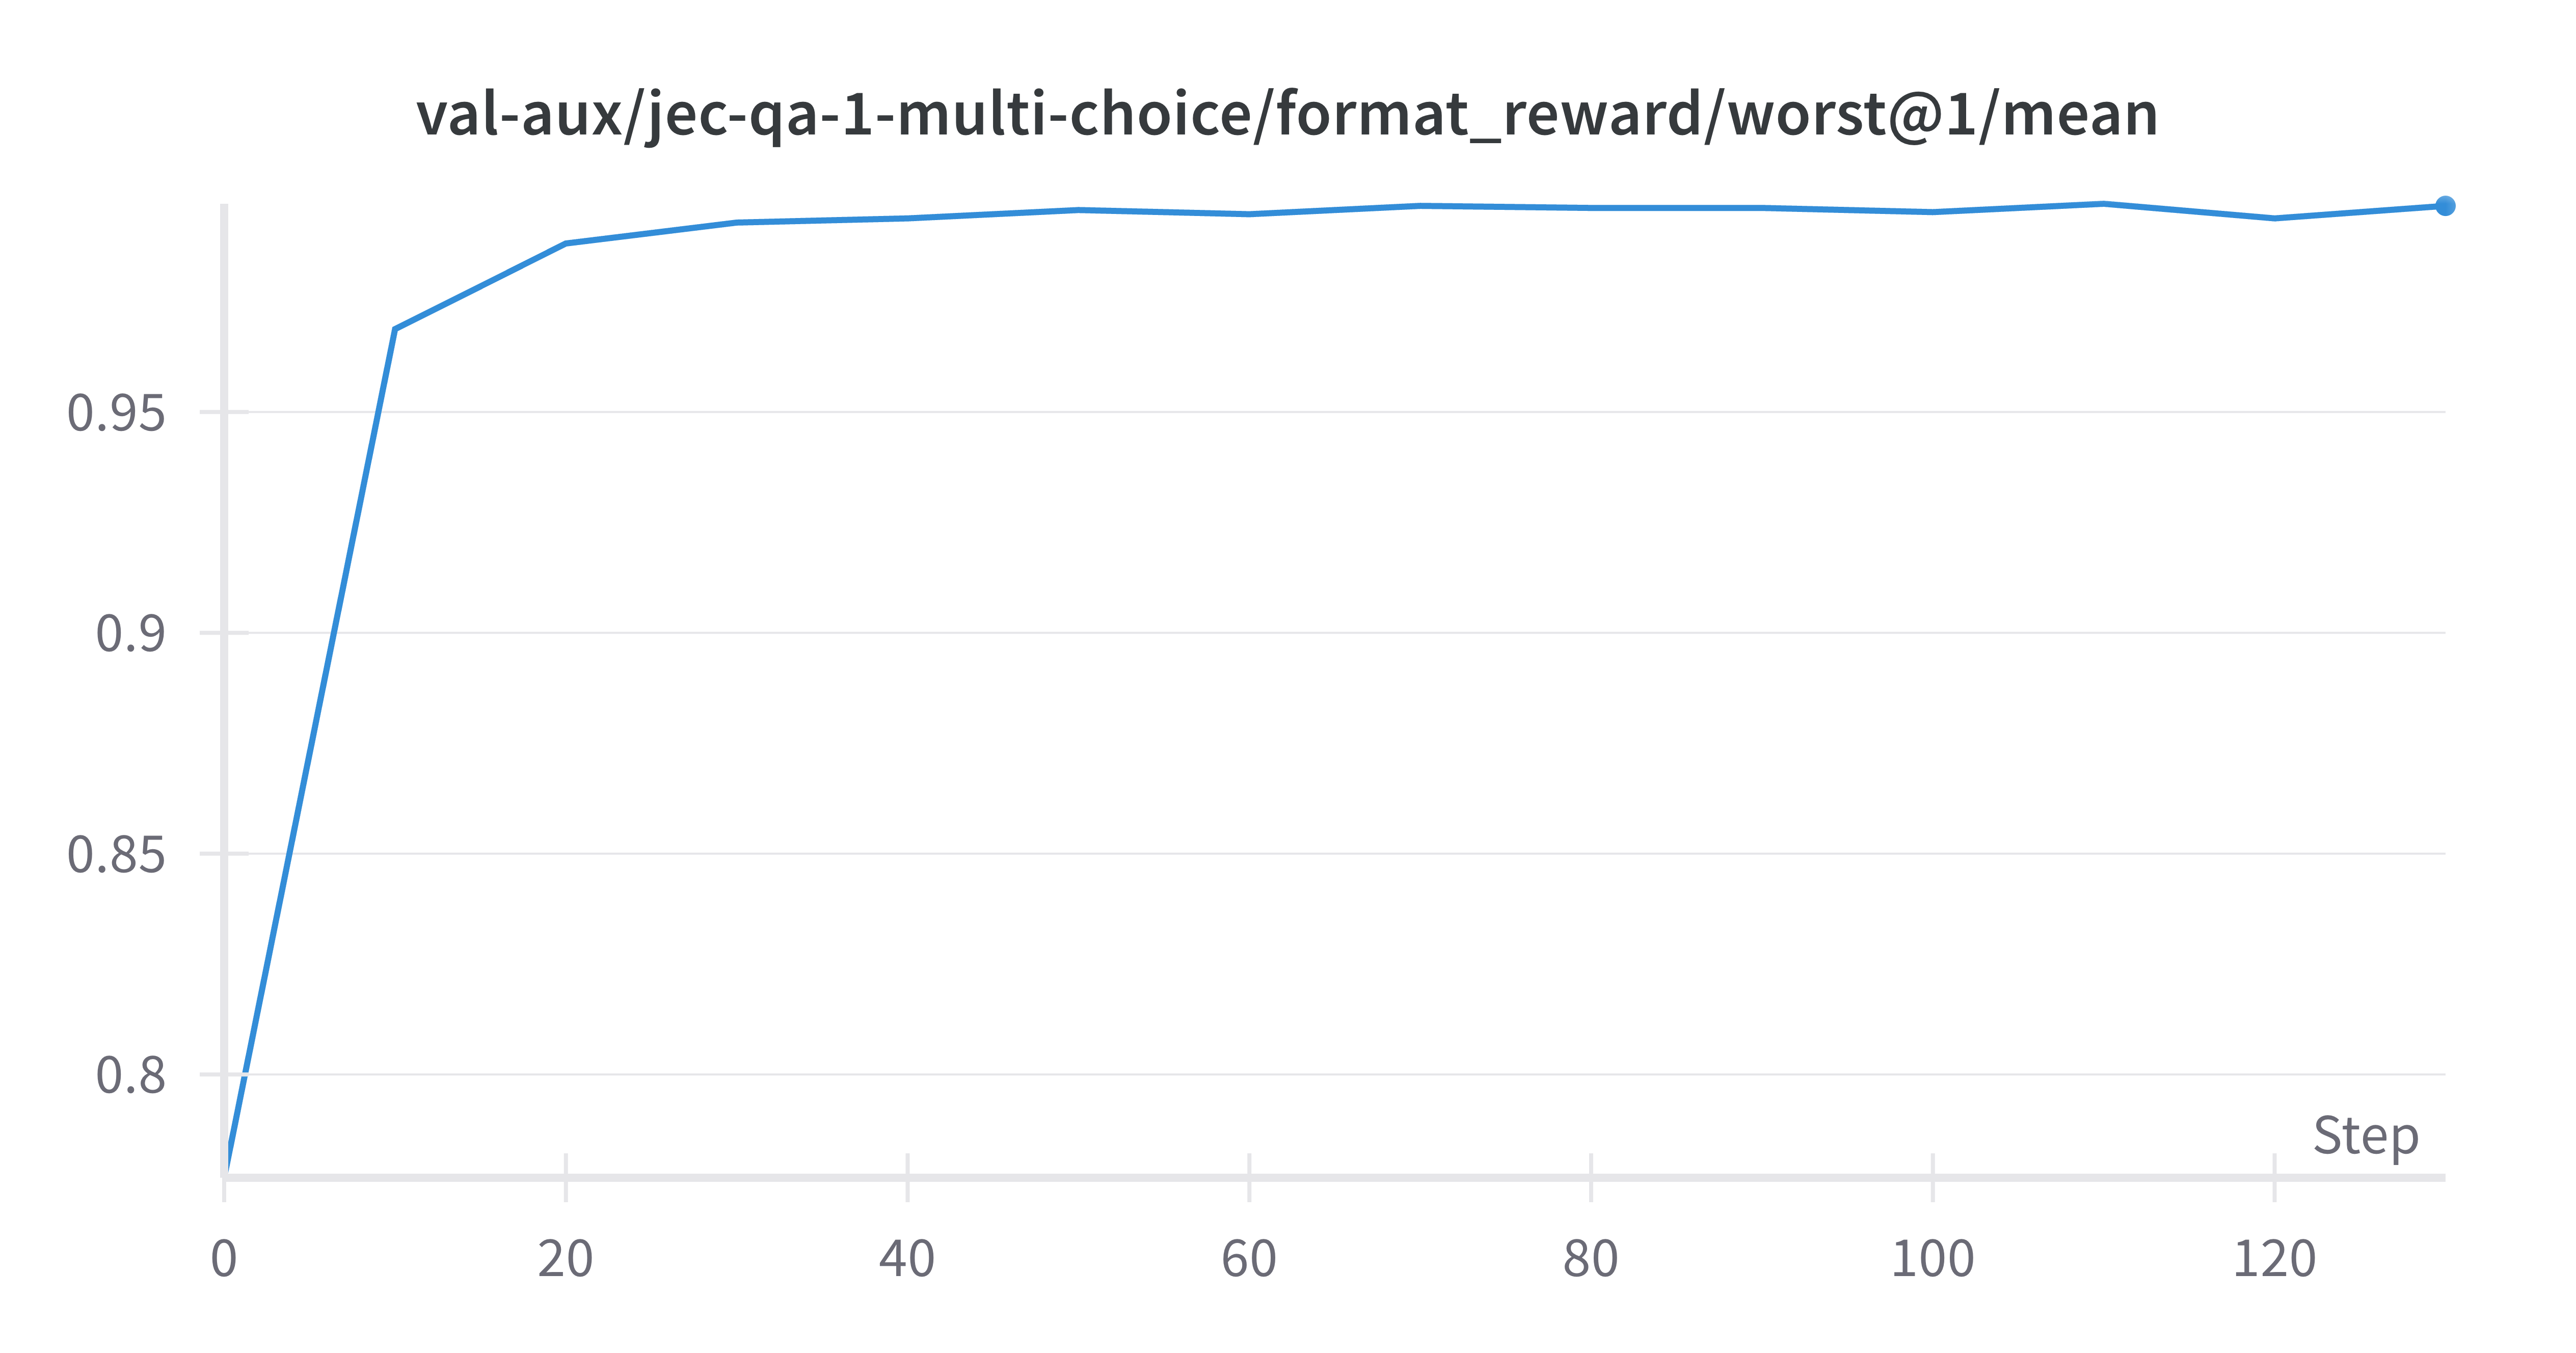
\includegraphics[width=0.8\textwidth]{figures/format.png}
\caption{移除格式奖励后模型准确率(Exact Match mean@1)随训练步数的变化情况}
\label{fig:format}
\end{figure}

尽管上述分析揭示了移除格式奖励后准确率的微降,但考虑到格式奖励在加速模型早期学习特定输出结构方面的积极作用(如表1所述),以及在我们的最终应用场景中,结构化的输出对于可解释性和用户体验至关重要。因此,在权衡了早期收敛速度、输出结构规范性以及对推理能力潜在的轻微影响后,我们的最终奖励函数选择整合了准确性奖励和格式奖励:
\begin{equation}
R = R_{\mathrm{accuracy}} + R_{\mathrm{format}}.
\end{equation}
其中,$R_{\mathrm{accuracy}}$ 可以是 $R_{\mathrm{exact}}$ 或 $R_{\mathrm{partial}}$,具体选择取决于特定实验阶段的侧重点。

\subsection{Zero-RL:无监督微调(SFT)的强化学习探索}
\label{sec:zero_rl_revised}
为了探究强化学习(RL)是否能够直接提升预训练模型在法律推理任务上的能力,而无需任何有监督微调(Supervised Fine-Tuning, SFT)作为预热阶段,我们尝试将 GRPO (Generalized Reinforcement Learning from Online Preference Optimization) 和 Dr.GRPO (Denoising Reward GRPO) 算法直接应用于 \qwen 模型。
\begin{itemize}
    \item \textbf{实验目的:} 核心目的是评估在不经过SFT的情况下,RL算法能否从零开始有效地优化模型在复杂法律推理任务上的表现。
    \item \textbf{实验结果:} 结果表明,这种"从零开始"的强化学习(Zero-RL)方式对于\qwen 这样规模的基础模型,在特定任务和奖励设计下表现出较高的学习效率。模型的收敛速度较快,并且在推理准确率上的提升非常显著,达到了58.2\%的水平。这一重要发现揭示了对于复杂的法律推理任务,即使缺乏SFT阶段的领域知识和任务模式初步对齐,较小参数量的基础模型仍然可能通过RL算法直接进行高效探索和学习,并达到与更复杂训练流程相当的性能。
\end{itemize}

\subsection{SFT + RL:基于蒸馏数据的冷启动策略}
\label{sec:sft_rl_revised}
除了直接应用强化学习(Zero RL)并观察到其高效性外,我们还探索了另一种主流的后训练范式,即"监督微调 + 强化学习"(SFT + RL)的多阶段训练策略。此路径旨在研究SFT作为RL的"冷启动"阶段,能否为模型在学习稳定性、对特定输出质量(如结构性)的控制,或在不同评估维度上带来与Zero-RL相比的差异化优势。我们通过知识蒸馏的方式为SFT阶段提供高质量的训练数据。

\paragraph{蒸馏数据准备:}
我们采用了由 \deepseekr 模型在 JEC-QA (Judicial Examination Comprehension Question Answering) 数据集上生成的思维链(Chain-of-Thought, CoT)响应作为SFT阶段的蒸馏数据。选择 \deepseekr 是因为其在相关任务上已展现出较强的推理和生成能力,其CoT响应能够为我们的目标模型提供高质量的推理示范。

\paragraph{详细训练流程:}
整个训练流程分为SFT阶段和RL(GRPO)阶段:
\begin{itemize}
    \item \textbf{SFT 阶段:}
    \begin{itemize}
        \item \textbf{基础模型:} \qwen。
        \item \textbf{主要训练参数:} 训练进行了 2 个周期(epoch),批处理大小(batch size)设置为 32,学习率(learning rate)采用 $1 \times 10^{-5}$,上下文长度(context length)限制为 1024 tokens。
        \item \textbf{SFT效果:} 通过在该蒸馏数据上进行SFT,模型的精确匹配率(mean@1)从初始的 29.5\%(\qwen 在该任务上的zero-shot或few-shot基线性能)显著提升至 42.4\%。这证明了SFT在快速引导模型适应目标任务和数据分布方面的有效性,为后续的RL阶段提供了一个更高性能的起点。
    \end{itemize}
    \item \textbf{GRPO 强化学习阶段:}
    \begin{itemize}
        \item \textbf{奖励函数配置:} 在此阶段,我们同时使用了前述定义的完全匹配奖励($R_{\mathrm{exact}}$)和格式奖励($R_{\mathrm{format}}$)来指导模型的学习。
        \item \textbf{主要训练参数:} Token截断长度设置为 1024,GRPO算法中的裁剪比率(clip ratio)初始值设为 0.6。
        \item \textbf{GRPO效果:} 经过GRPO阶段的强化学习,模型的精确匹配率(mean@1)从SFT后的 42.4\% 进一步提升至 58.2\%。
    \end{itemize}
\end{itemize}

\paragraph{不同训练阶段性能对比:}
为了更清晰地展示多阶段训练的效果,并与Zero-RL的结果进行参照,我们分析了模型在不同训练策略和阶段于验证集上的准确率表现。

\begin{table}[h]
\centering
\caption{不同训练策略及阶段模型在验证集上的准确率对比(mean@1)}
\label{tab:acc_distill_sft_grpo_revised} % Changed label to reflect revision
\begin{tabular}{l|c}
\hline
模型/训练阶段 & 准确率 (mean@1) \\
\hline
\qwen (Zero-Shot Baseline) & 29.5\% \\ % Added baseline for clarity
\qwen (Zero-RL, GRPO) & 58.2\% \\ % Added Zero-RL result here
\hline
\deepseekr (教师模型,参考性能) & 67.4\% \\
\qwen (SFT后,蒸馏自\deepseekr) & 42.4\% \\
\qwen (SFT + GRPO, 1024 tokens 上下文) & 58.2\% \\
\qwen (SFT + GRPO, 4096 tokens 上下文) & 50.9\% \\
\hline
\end{tabular}
\end{table}

从表 \ref{tab:acc_distill_sft_grpo_revised} 的数据可以看出,直接对 \qwen 模型进行Zero-RL(采用GRPO算法)能够使其精确匹配率从29.5\%的基线水平大幅提升至58.2\%。
在SFT+RL的流程中,SFT阶段首先为模型带来了显著的初始性能提升(从29.5\%提升至42.4\%)。随后的GRPO强化学习阶段进一步将此性能优化至58.2\%。
对比可见,Zero\-RL路径和SFT+RL路径最终均达到了相似的高性能水平(58.2\%)。这表明,对于\qwen 这一7B规模的模型,在此特定法律推理任务和奖励设置下,直接RL和SFT后进行RL均是可行的优化路径。
值得注意的是,在SFT+RL流程中,当我们将GRPO训练和评估时的上下文Token长度从1024扩展到4096时,性能反而有所下降(从58.2\%降至50.9\%)。这可能与模型在较长上下文中有效捕捉和利用信息的能力有关,或者是由于训练与推理时上下文长度不一致所带来的分布偏移。尽管两种RL路径最终性能相当,且相较于仅SFT有显著提升,但学生模型与教师模型 \deepseekr 之间本身存在一定的能力差距,其性能仍未达到教师模型的水平。

\subsection{结构性增强与案例分析}
\label{sec:structural_enhancement_revised}
除了关注准确率等硬性指标外,我们还深入分析了不同训练阶段(特别是SFT后以及Zero-RL和SFT+RL后)模型生成响应的结构性特征,旨在进一步评估不同强化学习策略对模型输出质量的综合提升效果。良好的结构性不仅能提升响应的可读性和可理解性,也是衡量模型是否能生成高质量法律文书的关键。

\begin{itemize}
    \item \textbf{结构性评估指标包括:}
    \begin{itemize}
        \item \textbf{编号段落的使用:} 是否倾向于使用有序列表(如1, 2, 3... 或 a, b, c...)来组织论点和解释。
        \item \textbf{逻辑连接词的频率:} 如"首先"、"其次"、"再次"、"综上所述"、"因此"、"然而"等有助于构建清晰逻辑流的词语的使用情况。
        \item \textbf{法规条文的引用与解释:} 是否能够准确且适当地引用相关的法律法规条文(即使是隐式依赖),并对其进行合理解释以支撑其论证。
        \item \textbf{解释性与分析性句式的出现:} 是否包含对案情细节、法律概念、选项合理性进行深入分析、辨析和阐释的句式,而不仅仅是简单罗列结论。
    \end{itemize}
    \item \textbf{RL阶段对结构性的影响:} 通过对比分析,我们发现经过GRPO强化学习阶段训练后的模型(无论是通过Zero-RL路径还是SFT+RL路径),在输出响应时均更倾向于生成具有清晰逻辑层次和良好组织结构的文本,相较于仅SFT的模型有明显改善。这具体表现为:
    \begin{itemize}
        \item \textbf{平均响应Token数增加:} 模型生成的解释和论证内容更为详尽和充实,提供了更丰富的上下文和推理细节。
        \item \textbf{逻辑衔接词使用更频繁且恰当:} 表明模型试图构建更连贯、更易于读者理解的推理过程。
        \item 从图 \ref{fig:grpo_distill_convergence_revised} 中所示的GRPO训练收敛曲线(例如奖励值的提升)可以间接推断,模型在优化奖励的同时,也在逐步学习和采纳那些能带来更高奖励的输出模式,而这些模式往往与更清晰的结构和更强的推理相联系。
    \end{itemize}
    \item \textbf{案例分析:} 对具体案例的模型输出进行人工检查和定性分析显示,经过RL优化后的模型所生成的推理链条,不仅在形式上更好地遵循了预设的"思考-回答"模式,在内容和语言风格上也更贴近于司法实务中的专业表达。例如,模型能够更自然地组织多角度论点、更细致地阐述每个选项的判断理由,并展现出更强的逻辑一致性。Zero RL和SFT+RL在这些定性方面的表现相似,均优于仅SFT的模型。
\end{itemize}

\begin{figure}[h]
\centering
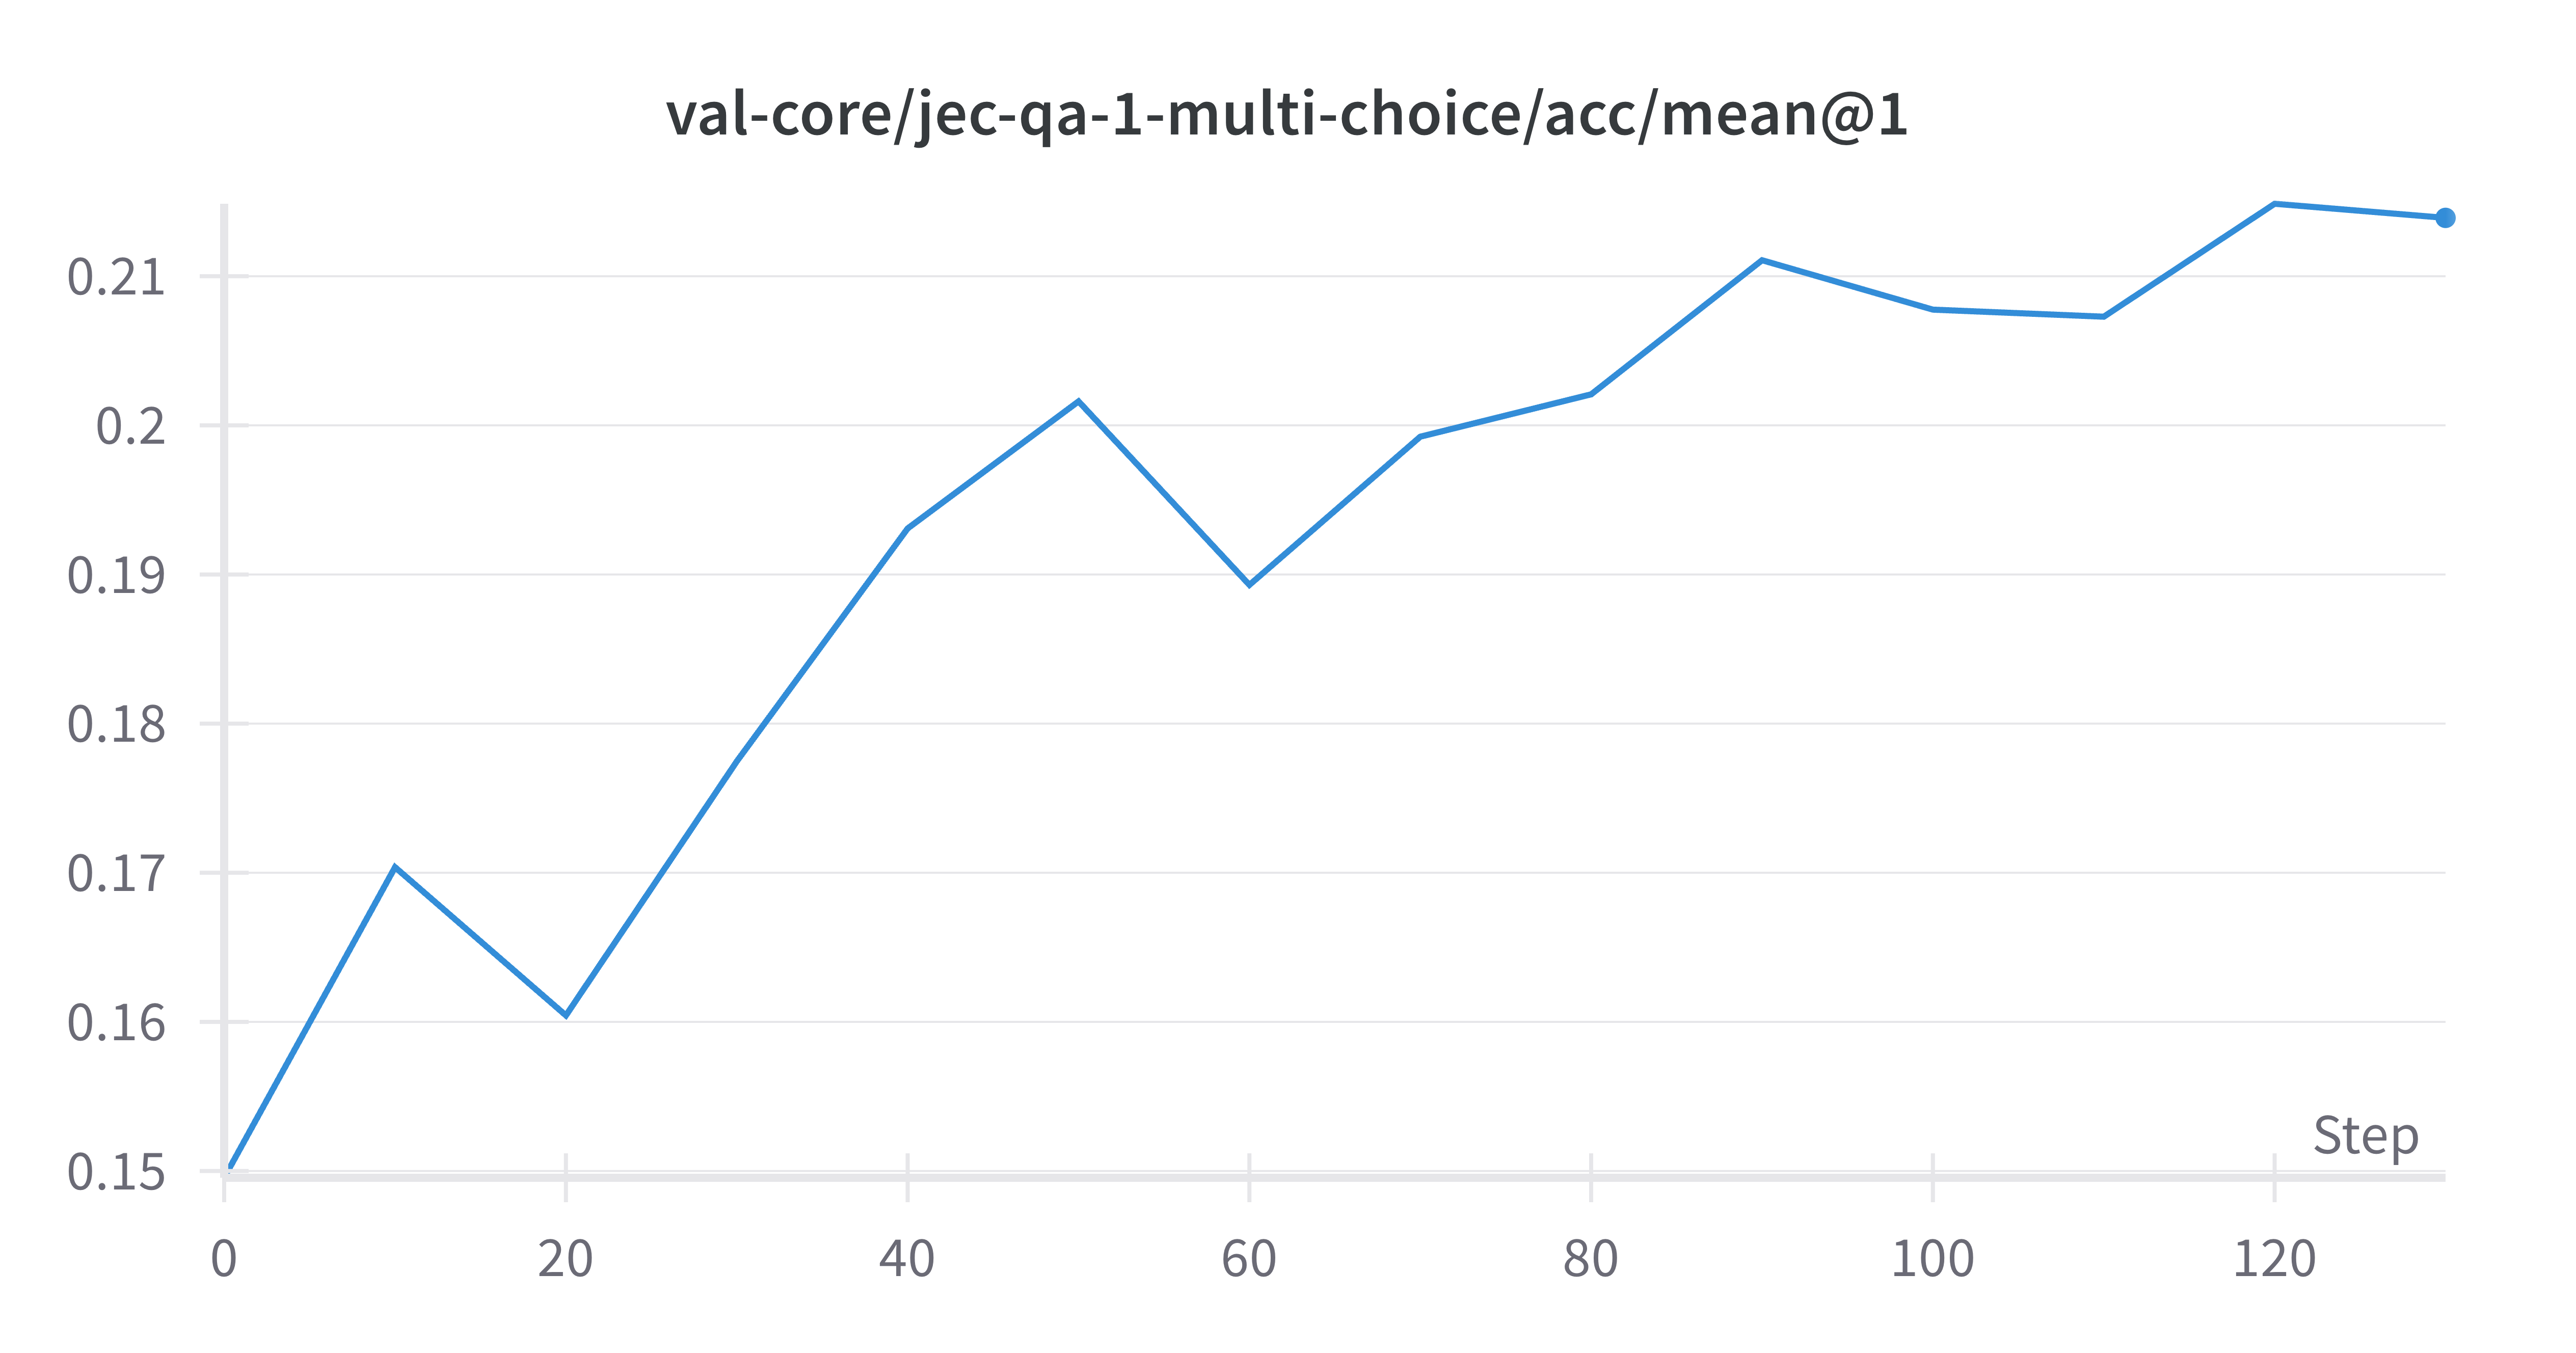
\includegraphics[width=0.8\textwidth]{figures/GRPO_DeepSeek-R1-Distill-Qwen-7B.png} % User provided path
\caption{GRPO 阶段训练收敛曲线(例如,平滑后的奖励或准确率)以及伴随的结构性增强趋势示意 (此图可能代表SFT+GRPO路径的收敛情况;Zero-RL路径也经历类似GRPO优化过程)}
\label{fig:grpo_distill_convergence_revised} % Changed label
\end{figure}

\paragraph{本章结论:}
\label{sec:chapter5_conclusion_revised}
综合上述实验设计与结果分析,我们可以得出结论:对于提升 \qwen 模型在法律多选推理任务上的综合性能,直接应用强化学习(Zero-RL,使用GRPO)和采用"知识蒸馏辅助SFT,继以GRPO强化学习优化"的多阶段训练策略均是有效的路径,两者均能将模型的精确匹配率提升至约58.2\%的较高水平。这表明,即使对于未经过特定领域SFT的小型基础模型,通过精心设计的奖励函数和RL算法,也可能直接激发其在复杂专业任务上的潜力。
SFT+RL路径中,SFT阶段为后续RL奠定了坚实的知识基础并提升了起点,而RL阶段则进一步优化性能。同时,Zero-RL路径的成功为大模型训练策略提供了更灵活的选择,尤其是在SFT数据获取困难或成本较高时。
两种RL路径均显著提升了模型输出的准确性,并且在结构化表达能力与推理准确性之间取得了良好的平衡。RL通过奖励机制引导模型优化其决策逻辑和输出质量,特别是在生成内容的逻辑性、专业性和结构规范性方面带来了积极影响。这些发现为在专业领域应用和优化大语言模型提供了有价值的实践指引和新的视角。

\section{总结与展望}
\label{sec:conclusion_future_work_revised} % Changed label

\subsection{研究总结}
本研究系统地探讨了如何通过后训练策略,提升大语言模型在复杂法律多项选择题推理任务中的性能。我们以中国国家司法考试(JEC-QA)的案例分析型多选题为研究对象,采用 \qwen 作为基础模型,并以 \deepseekr 作为教师模型进行知识蒸馏(用于SFT+RL路径)。

主要研究成果包括:
\begin{enumerate}
    \item \textbf{强化学习路径的有效性验证:} 实验结果清晰表明,无论是直接对预训练模型进行强化学习(Zero RL),还是采用"SFT + RL"的多阶段训练框架,均能显著提升模型性能,远超单一SFT(42.4\%)或Zero-Shot基线(29.5\%)的水平,最终均达到了约58.2\%的精确匹配率。
    \item \textbf{Zero-RL的潜力揭示:} 与传统认知中RL高度依赖SFT预热不同,本研究发现,对于\qwen 这一7B规模的基础模型,在JEC\-QA法律推理任务上,直接应用GRPO进行Zero\-RL训练,能够使其性能达到与更复杂的SFT+RL流程相当的高度。这为大模型训练策略,特别是在SFT资源受限情况下的优化,提供了新的思路。
    \item \textbf{SFT在多阶段训练中的作用:} 在SFT+RL路径中,通过高质量蒸馏数据进行的SFT,有效地为模型注入了领域知识,将基线性能从29.5\%提升至42.4\%,为后续RL阶段提供了一个更优的起点,并最终同样达到了58.2\%的精确匹配率。
    \item \textbf{奖励函数设计的关键作用:} 我们设计并评估了包括完全匹配奖励、部分匹配奖励及格式奖励在内的多种奖励函数。实验表明,合理的奖励函数设计(例如,选择适当的惩罚系数或侧重完全匹配)是RL成功的关键。格式奖励对早期学习速度和输出结构规范性的贡献,使其成为最终奖励函数中的有益组成部分。
    \item \textbf{RL对输出结构和质量的增强:} 除了准确率的提升,定性和定量分析均显示,GRPO强化学习(无论在哪种路径下应用)能够显著改善模型输出的结构性。模型更倾向于生成逻辑清晰、论证详细、语言风格更专业的响应。
\end{enumerate}
本研究为在法律等专业领域应用和优化大语言模型提供了一套行之有效的技术路径和实践经验,并对不同训练策略的潜力和适用性进行了有益的探索。

\subsection{研究贡献}
% This subsection seems fine as is, as it describes the general contributions.
本研究的主要贡献可以概括为:
\begin{itemize}
    \item \textbf{方法论层面:} 提出并成功实践了多种适用于法律领域复杂推理任务的大语言模型后训练方法,包括Zero-RL和SFT+RL,并通过知识蒸馏有效提升了SFT阶段的效率和效果。
    \item \textbf{实证层面:} 在具有代表性的中文法律推理数据集JEC-QA上进行了全面的实验验证,量化了不同训练策略和奖励机制对模型性能的具体影响,为后续研究提供了坚实的基准和参考。
    \item \textbf{技术洞察:} 深入分析了强化学习(特别是GRPO)在提升模型准确性和输出结构化表达方面的双重作用,并探讨了不同训练路径(Zero-RL vs SFT+RL)的有效性及奖励函数设计、上下文长度等因素对模型性能的影响。
\end{itemize}

\subsection{局限性分析}
% Modifying point 1 based on the new results.
尽管本研究取得了一些积极成果,但也存在以下局限性:
\begin{enumerate}
    \item \textbf{与教师模型的性能差距:} 尽管通过Zero-RL或SFT+RL策略均取得了显著提升(达到58.2\%),但学生模型 \qwen 的最终性能仍与教师模型 \deepseekr (67.4\% mean@1)存在差距。这表明在模型能力、蒸馏效率或RL优化方面仍有提升空间。
    \item \textbf{上下文长度敏感性:} 实验观察到,在SFT+RL的GRPO阶段将上下文长度从1024 tokens增加到4096 tokens时,模型性能出现下降。对于Zero-RL路径是否也存在类似敏感性未在本文中详细探讨。这表明模型在更长上下文中有效利用信息和保持推理一致性方面仍面临挑战。
    \item \textbf{奖励函数的依赖性与泛化性:} 当前的奖励函数主要基于规则(完全匹配、格式等)。虽然有效,但可能未能捕捉到法律推理中更细微、更主观的质量维度(如论证的深度、逻辑的巧妙性等)。未来可能需要结合人类偏好数据训练更复杂的奖励模型。
    \item \textbf{任务与数据集的特定性:} 本研究主要聚焦于法律多项选择题。研究结论在其他类型的法律任务(如案件摘要、法律咨询、文书生成等)或其他专业领域的适用性仍有待进一步验证。Zero-RL的有效性也可能与任务特性、模型规模和基础模型能力相关。
    \item \textbf{计算资源需求:} 大语言模型的SFT和RL训练,特别是使用GRPO这类需要多次前向传播的算法,对计算资源的需求较高。比较Zero-RL和SFT+RL在达到相似性能时的总计算成本和收敛速度,是未来值得研究的方面。
\end{enumerate}

\subsection{未来展望}
% This subsection seems fine as is, but the success of Zero-RL might add a nuance.
基于本研究的发现和局限性,未来可以从以下几个方面展开进一步的研究:
\begin{enumerate}
    \item \textbf{深入理解Zero-RL的机制与泛化性:} 针对Zero-RL在特定小型模型上表现出色的现象,深入探究其背后的机制,以及这种有效性是否可以推广到其他模型、其他任务或更大规模的模型上。比较Zero-RL与SFT+RL在训练动态、样本效率、鲁棒性等方面的差异。
    \item \textbf{更先进的RL算法与优化:} 探索和应用更先进的RL算法(例如对DAPO、Dr.GRPO等GRPO变体的深入实践和调优),或者针对法律推理任务的特性对现有算法进行改进,以期进一步提升训练效率和模型性能。
    \item \textbf{精细化的奖励模型:} 研究如何构建更精细化的奖励模型,例如通过收集法律专家的偏好数据来训练能够评估推理逻辑深度、论证质量、法律依据准确性等复杂维度的奖励函数,从而引导模型学习更高层次的法律推理能力。
    \item \textbf{长上下文处理能力的提升:} 针对模型在长上下文场景下性能下降的问题,探索专门针对长文本的建模技术(如更高效的注意力机制、分层处理等)和训练策略。
    \item \textbf{知识增强与可解释性:} 研究如何将外部法律知识库(如法律法规、判例数据库)更有效地融入LLM的训练和推理过程中,例如结合检索增强生成(RAG)技术,并提升模型决策过程的可解释性和可追溯性,使其符合TRACER标准。
    \item \textbf{跨法律任务与多模态融合:} 将本研究的方法和经验推广到更多样化的法律任务中,并探索融合文本、语音、图像等多模态信息的法律智能应用。
    \item \textbf{高效训练与推理框架的持续优化:} 持续关注并利用如VeRL、vLLM等高效训练和推理框架的最新进展,降低大模型在专业领域应用的门槛和成本。
\end{enumerate}
总之,通过不断的技术创新和跨学科合作,大语言模型在法律智能领域的应用潜力巨大。我们相信,未来的研究将推动AI在辅助立法、司法、普法以及法律服务等各个方面发挥越来越重要的作用,最终促进法治社会的进步。

\printbibliography

\Acknowledgments

大学四年,发生了太多事,有遗憾,有后悔,有开心,有失落。这四年是到目前为止最自由的四年,也是最迷茫的四年。在这即将踏出校园之际,我的思想、我的认知,与走进时截然不同。我往往丧失了对事物一体两面的看待,而总是会比较孰优孰劣,我总是会美化未曾踏足过的,而总是会贬低自己经历过的,我总是会活在过去,活在未来,而总是会忘记当下。
就像是Sisyphus一样,日复一日,年复一年,推着石头上山,又看着石头滚下山去,周而复始,永无止境。

我不再将这个世界与我所期待的,塑造的圆满世界比照,而是接受这个世界,爱它属于它,所谓的我,就是过去一切体验的总和,我是我接触过的人,创造过的物,感受过的情爱,迷失过的痛苦等等。所有的一切才成此刻的我,我唯一的事是爱这个世界,不藐视世界,不憎恶世界和自己,怀抱爱,惊叹和敬畏注视一切存在之物和我自己,世界并非不圆满,世间的每一瞬间皆未圆满,没有过去,没有未来,一切都是本具和当下。

在我十八岁时,我对未来,有着美好的憧憬,我对大学生活有着无比清晰的刻画,我以为我会坚定不移走向未来,但现实是,大部分时间里我充满了迷茫,十八岁前的生活,目标总是无比清晰,我曾常常抱怨为什么只有考试这一条路,只有分数这一个衡量标准,只有大学这一个目标,我期待大学后获得此生从未拥有的自由,广阔天地大有可为,但自由的代价是迷茫,是无所适从,是不知道自己想要什么,不知道自己该做什么,我花了四年时间认清我自己,我想要做什么,我想过上怎样的生活。我无权伦断他人的生活,唯独对自己的生活,必须做出判断。一步步纠错,一步步成长,感谢四年在北大的日子,余虽愚,卒终有所获。

Sisyphus:
挪威的森林 30 年

Sisyphus:
一体两面

Sisyphus:
活在未来 活在过去

Sisyphus:
美化从未踏足过的

Sisyphus:
这是最好的时代,也是最坏的时代


大学四年,有太多的人值得感谢。

首先,我要感谢我的导师冯岩松老师。冯老师在学术上严谨治学,在生活上平易近人,在科研上耐心指导,在论文上严格要求。

其次,我要感谢我的父母,他们在我成长的道路上给予了我无尽的关爱和支持。

然后,我要感谢我的同学和朋友,他们在我遇到困难时给予了我无私的帮助和鼓励。






\end{document}
